%!TeX root = 4-ml.tex
\documentclass[main]{subfiles}

\begin{document}

\chapter{Statistical Learning of Adsorption Properties}
\vspace*{-1\baselineskip}

\section{Machine learning models}

In the field of nanoporous material study, machine learning (ML) models have been widely used to characterize various properties such as adsorption, transport, catalytic or mechanical properties. These models offer a means to replace time-consuming simulations with simpler calculations of key descriptors, thereby aiding in the prediction of desired properties. In other cases, they are used to describe the structure-property relationships learned by the ML model. However, it should be noted that machine learning cannot be considered as a silver bullet since its application requires a comprehensive understanding of the key variables that improves prediction accuracy. In this study, a machine learning model will be built to characterize the separation of xenon from krypton at ambient pressure, utilizing the work on thermodynamic descriptors and knowledge on the effect of pressure on selectivity from the previous chapters.

\subsection{From algorithm to machine learning}

To understand the learning process of machines, it is necessary to understand how computers perform tasks. The human operator plays a key role in this process by designing the solution based on theoretical considerations and creating a list of instructions, known as an algorithm, which outlines the required actions for the computer to achieve the desired outcome under specific circumstances. In the context of physical or chemical science, these algorithms typically articulate the different components of a theoretical model, such as solving equations without analytical solutions or expressions, and addressing probabilistic problems. The previous chapters presented such algorithms used for simulating adsorption processes. For instance, GCMC simulations are based on the statistical physics of phase equilibrium between a gas phase and an adsorption phase within a nanoporous material, and Monte Carlo models are used to replicate the statistics associated with the grand canonical ensemble. Energy sampling algorithms, along with the Widom insertion are additional examples illustrating how computers assist theoreticians in modeling systems under specific chemical and physical conditions.

Machine learning models are also based on algorithms, but their objective differs significantly from that of the above-mentioned examples --- they don't aim at providing comprehensive computational details based on established theoretical principles. As their name suggests, machine learning algorithms aim to learn underlying relationships within input data, enabling them to perform tasks autonomously. The machine learning (ML) algorithm serves as a set of instructions guiding the machine learning process. For instance, clustering algorithms can distinguish different classes of elements within a disordered dataset, leading to the emergence of new concepts. This type of machine learning algorithm is referred to as unsupervised learning, as the data is not pre-labeled, and the machine assists in uncovering the underlying structure. As unsupervised learning extends beyond the scope of this thesis, further details on this algorithm type will not be provided.  It is worth mentioning that supervised learning models are the focus of study, which learns the relationship between labeled data and the characteristics (features or descriptors) of a given dataset. Subsequently, these models can predict the label of unlabeled data based on their characteristics.

The focus of this thesis lies on the supervised learning model, which learns the relationship between labels and their characteristics (referred to as features or descriptors) from a given set of labeled data points, enabling the prediction of labels for unlabeled data based on their characteristics. As an example, predicting tomorrow's weather could involve using past weather data from similar dates to infer whether it will rain. The ML model's features comprise the weather history, while the target variable or label of the data corresponds to the future weather.

The distinctions between a standard algorithm and an ML algorithm can be illustrated by a fascinating board game called Go. This game is traditionally played by two players on a 19$\times$19 board, where each player places black/white pieces to gain control over the maximum number of boxes. Based on these simple rules, different algorithms have been developed to make computers play the game. The first Go program was written in the late ’60s to mimic the pattern recognition of Go players when estimating the ``score'' through an influence function,\autocite{zobrist1970feature} and from the ’80s to the beginning of the 21\ex{st} century the first Go programs capable of playing were released. These programs were based on simple alpha-beta search algorithms that sought to test every possible move (while pruning the less promising ones). While they worked well in other games like chess (IBM's Deep(er) Blue beat the world chess champion in 1995), these types of programs in Go were only at the level of a novice player. The difference in performance lies in the combinatorics of both games. Chess has a number of legal positions lower than $10^{47}$,\autocite{website_labelle} while Go has approximately $10^{171}$ legal positions.\autocite{Tromp_2007,github_tromp_go} The state space to explore in Go is incomparably greater, and an increase in computing power that improved the performance of chess-playing computers would not make a significant difference for Go. A drastic reduction in the space to be explored is required for a computer program to work. The biggest improvement came in 2007 when a Monte Carlo tree search was introduced by Couloms.\autocite{Coulom_2007} This algorithm uses heuristics to distinguish between good and bad moves based on human perception of the game. A probability of selection is assigned to the moves according to their potential (policy), and potential moves are randomly selected based on this probability. The average outcomes associated with a parent move provide the value of the move. The computer Go is now more efficient in evaluating moves using a Monte Carlo sampling, and it can now play with average amateur players although it is nowhere near surpassing them. Up until now, the algorithms have been based on human knowledge that the programmer implements directly in the computer using machine instructions. Statistics and randomness are used to guide the machine towards the best moves and reduce their predictability, but the statistics that identify the moves are based on human heuristics that are usually not generalizable. The revolutionary aspect brought about by machine learning in the field aims to improve the evaluation of these statistics using data from previously played games. By using a dataset of 30 million moves, Alpha Go is based on the same Monte Carlo tree search framework, but the formulas behind the probability of searching a move are replaced by a machine learning model called the ``policy network'' and the evaluation of confidence in winning a position is done by a value ``network''.\autocite{Silver_2016} Alpha Go became the first computer program to beat a world champion in 2016. One year later, an improved version called Alpha Go Zero generated its own data by playing games against itself to train a similar machine learning structure as the one presented before. This new version beat the former version 100 times out of 100,\autocite{Silver_2017} marking a new era of computer dominance in Go over the world's best players, with the defeat of another top player further confirming the advent of this new era.

This example showed how the value of each move was learned by the machine through the compilation of knowledge from large datasets in a deep neural network. The main difference between conventional approaches to algorithmic and machine learning is very well illustrated in the previous example. The objective is not to instruct the computer on how to play using player knowledge implemented in formulas and explicit instructions. Instead, an explicit framework with flexible parameters is provided to the model, which needs to learn these parameters using a database. In other words, the model's parameters are adjusted to match the values of a database while having the ability to generalize to situations outside of the database (further discussion on the notion of generalizability will be presented in the following sections). The purpose of this section is not to provide a comprehensive overview of all existing models, but rather to introduce the main concepts of ML through the example of the model used in this thesis for the prediction of selectivity performance.

\subsection{Introduction to supervised learning}

In this thesis, the focus will be on the most common way to statistically learn from data, which is known as supervised learning. As previously introduced, supervised learning entails the extraction of a relationship between the labels of a set of data points and some of their known characteristics or features. This relationship can be referred to as the model or the predictor and is expected to generalize to similar but unseen data. In this section, the goal of the learning algorithm will be formalized when provided with a set of labeled data, to introduce more complex notions in machine learning, such as the bias--variance trade-off, as well as more specific models used in this chapter like the tree-based models. Various books have been consulted to develop this section, primarily the Elements of Statistical Learning\autocite{Hastie_2009} and an Introduction to machine learning (in French) from Azencott\autocite{azencott2022introduction}.

\subsubsection{Theoretical considerations}

In supervised learning, the algorithm learns from a set of data denoted as $\mathcal{D}_{n}=\left\{(\mathbf{x}_{1},y_{1}),...,(\mathbf{x}_{n},y_{n})\right\}$ with $n$ observed data points, where $\mathbf{x}_{i}$ represents an input observable, which is a vector of $\mathbb{R}^{p}$ ($p=1$ for scalars), and $y_{i}$ represents the label of the data point $i$ that belongs to a set $\mathcal{Y}$ (numerical, categorical or vectorial). 
The observed characteristics can be modeled by a random variable $X$, while the label is represented by another random variable $Y$. The dataset provides only a partial view of the joint probability (see equation~\ref{eq:joint_proba}), and the objective is to generalize the relationship to unseen data. $(X,Y)$ represents all possible combinations of seen and unseen data points.
\begin{equation}\label{eq:joint_proba}
  \forall\ \mathbf{x}\in\mathbb{R}^{p},\ y\in\mathcal{Y},\ \mathbb{P}\left(X=\mathbf{x}, Y=y\right) = \mathbb{P}(X=\mathbf{x})\mathbb{P}(Y=y|X=\mathbf{x})
\end{equation}
The challenge of supervised learning is that a complete picture of the probability law is not provided by the available data. The objective is to determine the most probable label $y$ for a given data point characterized by $\mathbf{x}$, which involves determining the conditional expectation $\E{Y|X=\mathbf{x}}$ of $Y$ given the observable $\mathbf{x}$. This determination relies on the conditional probabilities $\mathbb{P}(Y=y_i|X=\mathbf{x}_j)$ observed across all data points $i,j\in\{1,\ldots,n\}$.

\begin{figure}[ht]
  \centering
    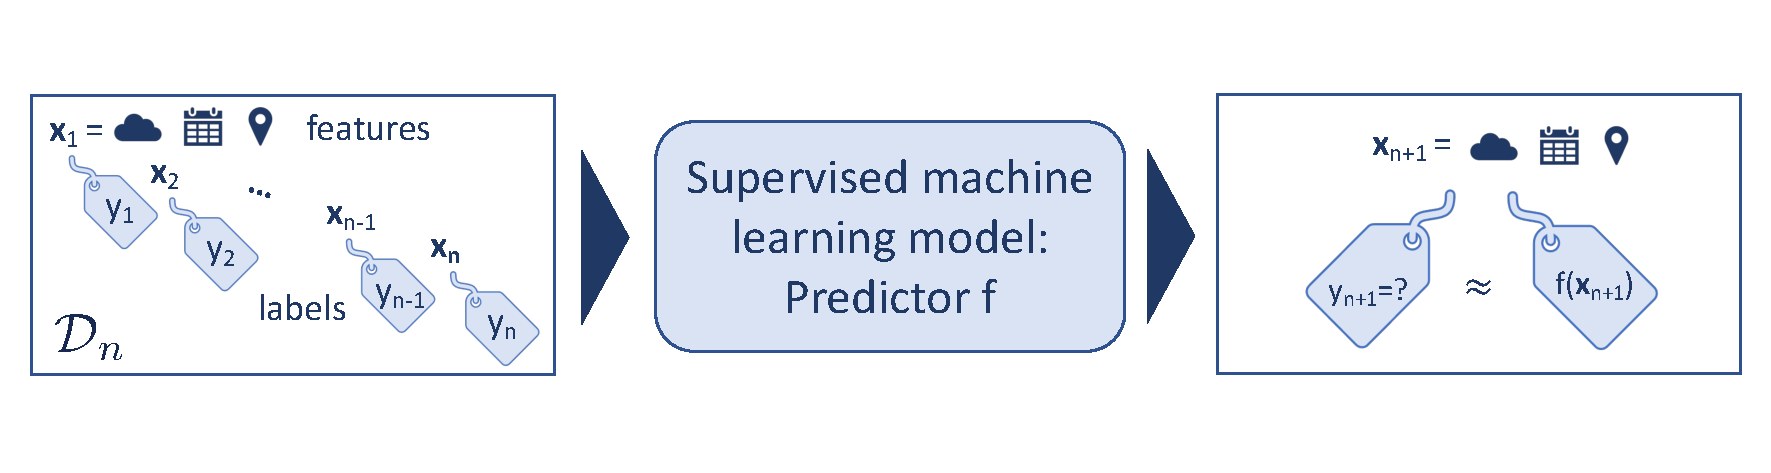
\includegraphics[width=0.9\textwidth]{figures/4-ml/machine learning.pdf}
    \caption{Illustration of the core principle of supervised learning. A data point of $\mathbb{D}_n$ corresponds to a set of features $\mathbb{x}_i$ labeled by $y_i$. The supervised machine learning model trains a predictor $f$ on the dataset $\mathbb{D}_n$ to predict unknown data $y_{n+1}$ using the features $\mathbb{x}_{n+1}$ so that $f(y_{n+1})\simeq y_{n+1}$ (approximate prediction).}\label{fgr:supervised_leaning}
\end{figure}

To achieve this, the learning algorithm uses a ``predictor'' $f$, which can be defined as the function that associates values (features) from $\mathcal{X}=\mathbb{R}^{p}$ with values from $\mathcal{Y}$. By changing the learning model (subsection~\ref{sct:model}) or the feature space $\mathcal{X}$, different domains $\mathcal{F}\subseteq{\mathcal{Y}}^{\mathcal{X}}$ where the prediction function $f$ is sought, can be defined. The domain $\mathcal{F}$ can be either too restrictive, resulting in the found optimal function being far from the theoretical one, or too large, making the optimization problem nearly impossible to solve or leading to a solution that is too close to the data. These issues raise questions regarding fitting, which will be discussed later.

This predictor can be interpreted as the function that provides the most probable outcome $y$ for a given input $\mathbf{x}$. To assess the quality of the predictor, a loss function $\mathcal{L}:\mathcal{Y}\times\mathcal{Y} \rightarrow \mathbb{R}^{p}$ is introduced to compare the predicted value $f(\mathbf{x})$ with the true value $y$ on available dataset $\mathcal{D}_{n}$. The loss function should increase when $f(\mathbf{x})$ deviates from $y$. To extend the definition of the loss to the entire possible space, the theoretical risk $\mathcal{R}$ of a predictor $h$ is introduced using the random variables $X$ and $Y$, such that $\mathcal{R}(h) = \E{\mathcal{L}\left(h(X),Y\right)}$. However, since the exact mapping of the random variables is unknown, the empirical risk $\mathcal{R}_n$ on the known dataset $\mathcal{D}_{n}$ is evaluated instead:
\begin{equation}\label{eq:risk}
  \mathcal{R}_n(h) = \frac{1}{n}\sum_{i=1}^n \mathcal{L}\left(h(\mathbf{x}_i),y_i\right)
\end{equation}

The goal, therefore, is to find a function that minimizes the risk function across the known data, and the optimal predictor $f^*$ can be defined as follows:
\begin{equation}\label{eq:min_f}
  f_n^* = \underset{f\in\mathcal{F}}{\text{arg min}} \mathcal{R}_n(f)
\end{equation}


The risk function can utilize various loss functions, with an increasing emphasis on large errors depending on their definitions. For instance, a quadratic cost function highly penalizes outliers, thus prioritizing a few medium errors over a single large error. Conversely, an absolute cost function does not exhibit this behavior. Since regression models were exclusively utilized in this thesis work, the details of classification loss functions will not be discussed extensively. Instead, the focus will be on regression loss functions. The quadratic loss or squared error loss $\mathcal{L}\e{SE}(f(\mathbf{x}),y)=0.5{\left(y-f(\mathbf{x})\right)}^2$ of a predictor $f$ on a data point $(\mathbf{x},y)$ is simply defined as the squared difference between the prediction and the true label. The multiplicative $0.5$ coefficient is included to simplify the derivatives. This loss is similar to the mean squared error (MSE) used to compare two quantities across a dataset, where the risk function corresponds to half of the MSE on the predictions $\mathcal{D}_n$:
\begin{equation}
  \mathcal{R}\e{SE}(f) = 0.5\frac{1}{n}\sum_{i=1}^n {\left(y_i-f(\mathbf{x}_i)\right)}^2
\end{equation}

A second commonly used loss function is the absolute loss, which is associated with the mean absolute error (MAE) utilized in error evaluation. The loss can be expressed as $\mathcal{L}\e{AE}(f(\mathbf{x}),y)=\left|y-f(\mathbf{x})\right|$, and the risk function associated with it is simply the MAE across the dataset predictions:
\begin{equation}
  \mathcal{R}\e{AE}(f) = \frac{1}{n}\sum_{i=1}^n \left|y_i-f(\mathbf{x}_i)\right|
\end{equation}
It is also possible to introduce a parameter $\epsilon$ to flatten loss function flatter near the minimal error. The $\epsilon$-insensitive loss corresponds to a modified absolute loss $\mathcal{L}_{\epsilon}(f(\mathbf{x}),y)=\max\left(0,\left|y-f(\mathbf{x})\right|\right)$.

Lastly, a Huber loss can be used to combine the less outlier-sensitive absolute loss with the smoothness of the quadratic loss near the minimal error domain. For a given $\delta$, the Huber loss is defined as:
\begin{equation}
  \mathcal{L}_{\delta}(f(\mathbf{x}),y) = \left\{
    \begin{array}{ll}
        \tfrac{1}{2}{\left(y-f(\mathbf{x})\right)}^2 & \mbox{for } \left|y-f(\mathbf{x})\right| \leq \delta \\
        \delta\left(\left|y-f(\mathbf{x})\right| - \tfrac{1}{2}\delta\right) & \mbox{otherwise.}
    \end{array}
  \right.
\end{equation}
A risk function $\mathcal{R}_{\delta}$ can also be determined using this loss function. The Huber loss is considered a robust loss function since it is less sensitive to the outliers (high values of error) and has a very smooth gradient near low error values like the squared error. It can be viewed as a combination of the advantages of both the absolute and squared errors as illustrated on Figure~\ref{fgr:loss_comp}.

\begin{figure}[ht]
  \centering
    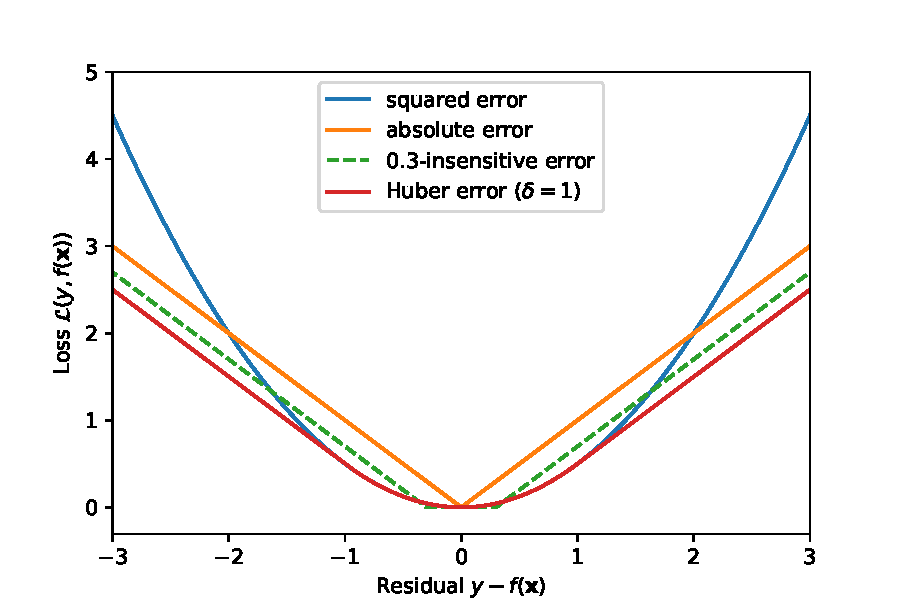
\includegraphics[width=0.6\textwidth]{figures/4-ml/loss_comparison.pdf}
    \caption{Comparison of different loss functions (quadratic loss, absolute loss, $\epsilon$-insensitive and the Huber loss). }\label{fgr:loss_comp}
\end{figure}

Through these theoretical considerations, the process of machine learning from data can hopefully be demystified by formulating this learning process as the optimization of a cost function, which is a common tool in any scientific field. However, this optimization problem poses challenges in the sense that the variable is a function that exists in a high-dimensional space, necessitating approximations to reduce the space. This is why most engineering breakthroughs occur in the conception of the architecture of the ML model, which defines the form of the prediction function $f$. Another difficulty in machine learning is dealing with an ill-posed problem, where one of the three conditions of Hadamard is not satisfied. These conditions pertain to the existence and unicity of a solution and its continuity with respect to the initial conditions. Typically, this issue is addressed through regularization techniques, such as the one introduced by Tikhonov in the second half of the 20\e{th} century. Furthermore, the minimization of the empirical risk does not always align with the minimization of the more global risk (considering all possible observations). In other words, minimizing $\mathcal{R}_n$ does not always yield the same solution as the minimization of $\mathcal{R}$. Therefore, the complexity of the risk optimization problem depends on the chosen loss function and the domain $\mathcal{F}$ defined by the model. Different techniques can be used to construct a solution without any guarantees of its optimality. One of the biggest challenges in ML is overcoming the problem of generalizability, which will be the topic of the next discussion. 


\subsubsection{Generalization and overfitting}

As previously discussed, the optimization problem is ill-defined and there is no guarantee the model will work on other data points as $n$ goes to infinite. The generalizability of model consists of ensuring the predictability of unseen data, where the solution does not only correspond to the minimal risk for the data $\mathcal{D}_{n}$ but also for other $m$ data points $\left\{(\mathbf{x}_{n+1},y_{n+1}),\ldots,(\mathbf{x}_{n+m},y_{n+m})\right\}$, all different from the previous set. One of the main phenomena that explain this discrepancy between the solution $f_n^*$ and the ideal solution $f^*$ (considering an infinite amount of data) is the noise in the dataset. The data is not perfectly measured, and the uncertainty attached to each $\mathbf{x}_i$ and $y_i$ values can create a residual noise that needs to be ignored in the learning process. Moreover, the $p$ explanatory variables considered are sometimes not sufficient to model the target phenomenon. To train a generalizable model, it is necessary to ensure sufficient learning to capture the inner relation between $X$ and $Y$ while avoiding fitting the data too closely and capturing the noise along the way. Otherwise, it is said that the model overfits the data. If the model is highly inaccurate even on the training data, it is said to underfit, generally indicating that the model is too simplistic (not enough features or too low-level architecture). 

This problem of overfitting can be summarized in the fundamental notion of bias--variance trade-off in machine learning and, more generally, in statistics. The error can be broken down in two types: the bias error measures the error made on the available data $\mathcal{D}_n$, while the variance error measures the sensitivity to small variations in the input values. A high bias error corresponds to underfitting, indicating that not enough is learned from the data. A high variance error corresponds to overfitting, indicating too much is learned, even including superfluous relations. To formalize these errors, reference can be made to the empiric risk function $\mathcal{R}_n(f)$ that models the error of the predictor $f\in\mathcal{F}$. To ascertain whether the ideal optimum has been achieved, a comparison with the minimal risk attainable by a predictor possessing infinite knowledge is necessary. This minimal risk is denoted as $\mathcal{R}^* = \underset{\scriptscriptstyle h\in\mathcal{Y}^{\mathcal{X}}} {\text{min}}\mathcal{R}(h)$. This excess error $\mathcal{R}_n(f)-\mathcal{R}^*$ can then be decomposed into two errors, which can be interpreted as the bias and the variance errors:
\begin{equation}\label{eq:generalization_error}
  \mathcal{R}_n(f)-\mathcal{R}^* = \left[\mathcal{R}_n(f) - \underset{\scriptstyle h\in\mathcal{F}} {\text{min}}\mathcal{R}_n(h)\right] + \left[\underset{\scriptstyle h\in\mathcal{F}} {\text{min}}\mathcal{R}_n(h) -\mathcal{R}^*\right]
\end{equation}
The first term of the above-written sum corresponds to a bias error, which measures the deviation between the current predictor $f$ and the minimum risk predictor $f_n^*$ (there can be multiple solutions in the case of an ill-posed problem) determined using the $n$ data points. The second term, on the other hand, is the residual error associated with the choice of the predictor domain $\mathcal{F}$  limited availability of data for the prediction model. In the presence of an infinite amount of data, the model $f^*$ associated with the risk $\mathcal{R}^*$ would not be influenced by the noise, as several data points with similar features but with minor noises would yield similar predictions. The difference in loss between this ideal function $f^*$ and the tested current function $f$ would correspond to an overfitting of the noise, which could not be distinguished in the finite case when the considering the domain $\mathcal{F}$ defined by the suitable model. Conversely, if there is a model issue, this error also measures the approximation error resulting from the selection of specific features and a particular model architecture.

\begin{figure}[ht]
  \centering
    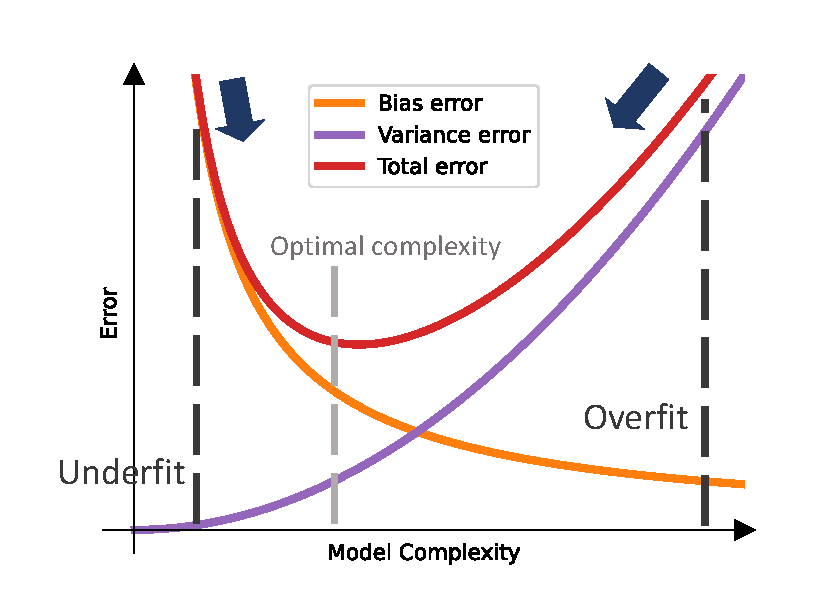
\includegraphics[width=0.45\textwidth]{figures/4-ml/Bias_variance_tradeoff.pdf}
    \hfill
    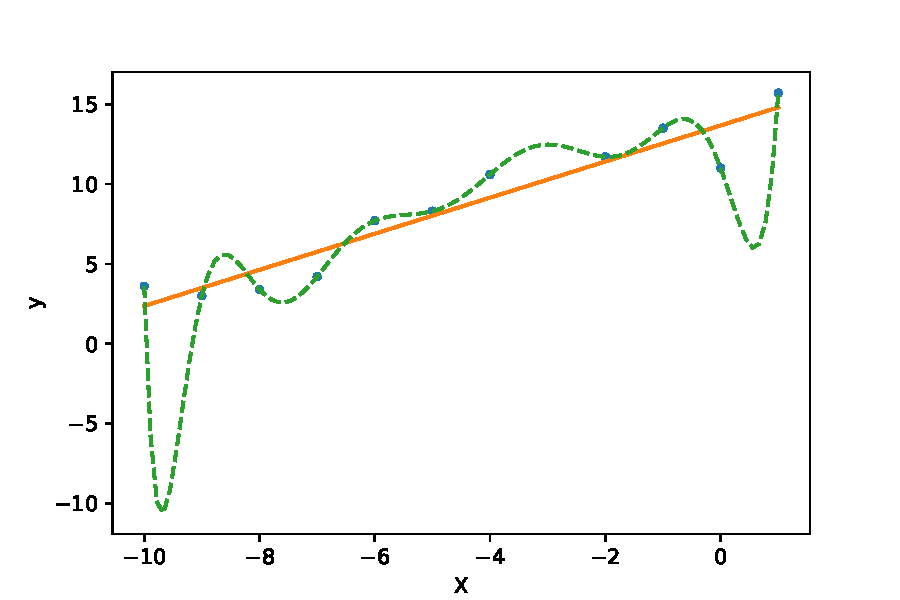
\includegraphics[width=0.45\textwidth]{figures/4-ml/overfit.pdf}
    \caption{On the left, theoretical relation between the bias, variance and total errors and the model complexity. The overfit case is illustrated on the right plot when considering polynomial fits. The lower degree linear function is more generalizable than the biased high degree polynomial that fits perfectly the data.}\label{fgr:bias_variance}
\end{figure}

In general, if the model is overly complex compared to the available data, it would result in a close fit to the data and a high risk of overfitting. Conversely, if the model is too simplistic, it would lead to a significant bias error and underfitting. This principle is depicted in Figure~\ref{fgr:bias_variance} and provides guidance for designing a new ML model.
The complex art of achieving an optimal fit between the model and the dataset involves finding the right balance between bias and variance. Fortunately, there are optimization techniques available that can help reduce the variance error by modifying the loss function itself. These tools will be discussed in the following section.

\subsubsection{Regularization to fight against overfitting}

Regularization consists generally in adding implicit or explicit constraints on the optimization problem to find not only the most accurate solution (minimal loss) but also the simplest solution. This criterion of simplicity is crucial for achieving generalization of the problem. A higher degree polynomial is typically unnecessary when a linear function is a more suitable solution, as demonstrated in Figure~\ref{fgr:bias_variance}. 

The explicit regularization technique consists in penalizing the complexity of a model by adding to the global loss function an error term that is scaled according to the complexity of the model. The error associated with a predictor $f$ can be expressed with an additional regularization term ${\Omega}_n(f)$:
\begin{equation}
  \mathcal{R}_n(f) = \frac{1}{n}\sum_{i=1}^n \mathcal{L}\left(f(\mathbf{x}_i),y_i\right) + \Omega_n(f)
\end{equation}
The influence of regularization on the optimization problem varies depending on the expression of the regularization term, denoted as ${\Omega}_n(f)$. 

Since the regularization is a model-specific function (depends on $f$), the definition of a model is necessary to explore more specific regularization expressions.
Consideration is given to a multilinear model $f(\mathbf{x}) = \boldsymbol{\beta}\mathbf{x}\ex{T}$, where $\boldsymbol{\beta}=(\beta^{(1)},\ldots,\beta^{(p)})$ is a vectorial representation of the weights of the $p$ features contained in $\mathbf{x}$ in the linear regression. In the case of standard multilinear regression with a quadratic loss, the risk function to be minimized can be expressed as follows:
\begin{equation}\label{eq:linear}
  \mathcal{R}_n(f) = \frac{1}{n}\sum_{i=1}^n {\left(\boldsymbol{\beta}\mathbf{x}_i\ex{T}-y_i\right)}^2 
\end{equation}
Here, $y_i$ represents a scalar quantity in a regression problem ($\mathcal{Y}=\mathbb{R}$). One of the earliest regularization tools introduced by Tikhonov to address ill-posed optimization problem is the L2 regularization. When used in linear regression, this novel model type, known as ridge regression, consists simply in adding a L2-norm penalty to the model weights within the risk function, as expressed by the following equation:
\begin{equation}\label{eq:L2_reg}
  \mathcal{R}_n(f) = \frac{1}{n}\sum_{i=1}^n \mathcal{L}\left(f(\mathbf{x}_i),y_i\right) + \lambda_2 {\lVert \boldsymbol{\beta} \rVert}_2^2 = \frac{1}{n}\sum_{i=1}^n {\left(\boldsymbol{\beta}\mathbf{x}_i\ex{T}-y_i\right)}^2 + \lambda_2 \sum_{k=1}^p \left|\beta^{(k)}\right|^2
\end{equation}
where $\lambda_2$ is the parameter of the L2-regularization that controls the importance of the regularization term in the optimization process. By adjusting this parameter, the complexity of the model can be regulated, aiming to find an optimal balance between accuracy and generalizability, as depicted in Figure~\ref{fgr:bias_variance}. In the case of considering a polynomial function, where the vector $\mathbf{x}_i$ represents various exponentiations of a scalar $x_i$, such that $\mathbf{x}_i=\left(x_i^0,\ldots,x_i^{n-1}\right)$, the coefficients $\boldsymbol{\beta}$ correspond to the polynomial coefficients of the function $f$. This serves as a clear illustration of how the regularization terms penalize the complexity of the model by directly penalizing the number of terms utilized and influence impact on the fitting process. It is worth noting that this regularization technique can be adapted to other types of models, provided that a suitable L2-norm of the prediction function $f$.

Another commonly used regularization term is based on the L1-norm of the prediction function. L1-regularized least square linear regression, known as LASSO (Least Absolute Shrinkage and Selection Operator) regression, allows for a sparser selection of the model weights by permitting certain weights to be zero in the model, unlike L2-regularization. The risk function associated with this regression model can be expressed as follows:
\begin{equation}\label{eq:L1_reg}
  \mathcal{R}_n(f) = \frac{1}{n}\sum_{i=1}^n \mathcal{L}\left(f(\mathbf{x}_i),y_i\right) + \lambda_1{\lVert \boldsymbol{\beta} \rVert}_1 = \frac{1}{n}\sum_{i=1}^n {\left(\boldsymbol{\beta}\mathbf{x}_i\ex{T}-y_i\right)}^2 + \lambda_1 \sum_{k=1}^p |\beta^{(k)}|
\end{equation}
where $\lambda_1$ is the L1-regularization parameter that controls its importance. The L1-norm can be defined in various ways depending on the model, but its fundamental concept revolves around being a function of the absolute values of the model weights.

Lastly, when both L1 and L2-regularization are combined, linear regression transforms into elastic net regression, and the risk function can be expressed as follows:
\begin{equation}\label{eq:elasticnet_reg}
  \mathcal{R}_n(f) = \frac{1}{n}\sum_{i=1}^n \mathcal{L}\left(f(\mathbf{x}_i),y_i\right) + \lambda_{1,2} \left({\alpha \lVert \boldsymbol{\beta} \rVert }_1 + (1-\alpha) {\lVert \boldsymbol{\beta} \rVert}_2^2\right)
\end{equation}
where $\alpha\in[0,\,1]$ defines the relative weight of L1 and L2 regularization terms, and $\lambda_{1,2}$ governs the importance of the combined regularization term. This regularization technique consists in simply combining both L1 and L2 regularization, and the different regularization parameters can be adjusted to find the optimal bias--variance trade-off for the final model. These parameters are also commonly referred to as hyperparameters in machine learning, as they influence the parameters at a higher level in the model.

Finally, implicit regularization encompasses alternative forms of controlling the complexity of the model. For instance, it can involve implementing early stopping during the learning process to avoid complete convergence to minimal error with the data. It can also include the removal of outliers that prevent the model from learning properly on relevant data. Furthermore, the architecture of the model itself can contribute to implicit regularization. For instance, random forests are based on an ensemble approach that aims at reducing overfitting, which will be discussed in the next section. The learning rate in gradient boosting is another regularization parameter that smooths the learning process and will be addressed in the dedicated section. Implicit regularization is related to the construction of the model and will therefore be elucidated in greater detail in the section on machine learning models.

\subsubsection{Learning strategies}

The theory behind the bias--variance trade-off has been previously introduced, emphasizing the generalization of a model that has a partial glimpse of the available data. However, in practical applications, it is necessary to evaluate the generalization error $\mathcal{R}_n(f)-\mathcal{R}^*$. This evaluation is achieved through a common strategy that consists in randomly splitting the available data into two sets: a training set $\mathcal{D}\ex{train}=\left\{{(\mathbf{x}_{i_1},y_{i_1}),\ldots,(\mathbf{x}_{i_N},y_{i_N})}\right\}$ and a test set $\mathcal{D}\ex{test}=\left\{(\mathbf{x}_{j_1},y_{j_1}),\ldots,(\mathbf{x}_{j_{n-N}},y_{j_{n-N}})\right\}$, such that $\mathcal{D}_n = \mathcal{D}\ex{train} \cap \mathcal{D}\ex{test}$. The training set is used to solve the optimization problem as defined in equations~\ref{eq:risk} and~\ref{eq:min_f}, while the test set is employed to assess the generalization error, as it comprises unseen data for the model. In practical applications, a ratio of test data $n-N/n$ (e.g.\ {20\%}) that defines the size of the test set from an initial dataset is chosen. The randomness of the split ensures that the data from both sets are similar, yet not identical. However, in some cases, it is important to acknowledge that outliers may be present in the test set in certain cases, thereby resulting in poorer performance than expected. In other cases where the dataset is small and individual data points exhibit significant dissimilarities, the test set may differ significantly from the training set, rendering it impossible for the model to make predictions based on the piecemeal information provided by the training set. Therefore, the percentage of the train/test split should be thoughtfully chosen to maintain representativeness of the training set.

The main property of the test set is that it is composed of an entirely unseen dataset, which means the training of the model should be independent of this set, except for the final evaluation. However, in some cases, different models need to be compared or a ``hyperparameter'' such as the regularization parameter within the same model architecture needs to be altered. To evaluate these models, the generalization error on the test set cannot be computed for each model, as it would compromise the independence of the test set from the training process. Therefore, validation sets are introduced within the initial training set. A simple training/validation split similar to the train/test split could be performed. Nevertheless, this approach would further weaken the model due to the reduced amount of available data. Moreover, it does not fully utilize the potential of the training set. One widely used technique to test the performance of a model on a training set is cross-validation. This method aims to test the model in multiple configurations by employing different training/validation splits, thereby providing a more comprehensive evaluation of the model's performance through averaging different performances. 

The most commonly used method is k-fold cross-validation, which consists in partitioning the training set $\mathcal{D}\ex{train}$ into k equal-sized subsets $\mathcal{S}_1,...,\mathcal{S}_k$. The model is then trained on the union $\bigcup_{l\neq m} \mathcal{S}_l$ of all subsets but one subset $\mathcal{S}_m$ that will be used as the validation set for all $m\in \{1,\ldots,k\}$. The principle of the k-fold approach is illustrated in Figure~\ref{fgr:kfold}. The approximate generalization error of the model is then computed as the average of the losses calculated on the validation subsets. This tool provides a method for comparing different models without using the test set, which is extremely useful, especially in the parameterization of the ML model.

\begin{figure}[ht]
  \centering
    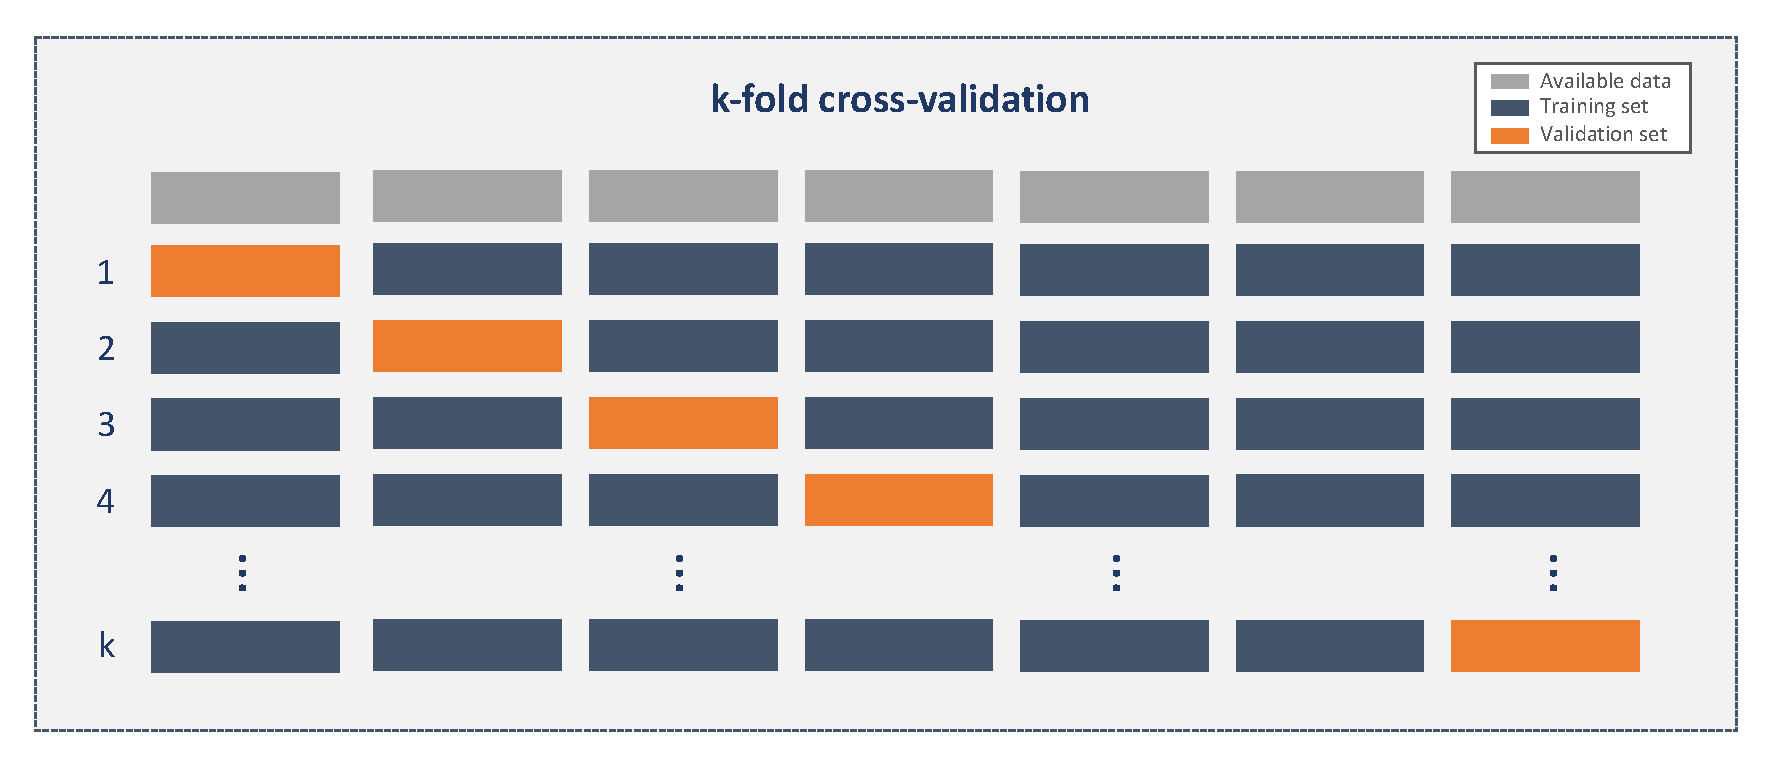
\includegraphics[width=0.8\textwidth]{figures/4-ml/cross-validation.pdf}
    \caption{Illustration of a k-fold cross-validation. At each step, the machine learning model learns from the training set and is tested on the validation set. The average performance on all validation sets gives an approximation of the generalization error.}\label{fgr:kfold}
\end{figure}

Other cross-validation techniques exist and are used in specific cases. For instance, stratification cross-validation ensures the same distribution of labels $y_i$ in each subset, which is particularly useful for classification problems. Increasing the value of k in  k-fold validation can make the validation process even more exhaustive. However, this approach requires training the models k times, resulting in an increased computation time. When k reaches the maximum value equal to the size of the training set, the method is referred to as leave-one-out cross-validation. In the case of time series data, the cross-validation technique typically involves sorting the data based on the time history, ensuring that the training set always precedes the validation set. This introduces a completely novel approach to cross-validation. The fundamental concept behind cross-validation is to find multiple training/validation splits to evaluate the model from various points of view. Different strategies exist depending on the specific training problem at hand.

\subsection{Machine learning models}\label{sct:model}

In this chapter, the transition will be made from the basic components of the model (decision tree) to the more complex ensemble model (e.g.\ random forest), ultimately concluding with the final stochastic gradient boosting model used in this work. The focus of the discussion will primarily revolve around regression problems rather than classification problems, as the objective is to predict a continuous variable (the xenon/krypton selectivity).

\subsubsection{Regression tree}

Tree-based models are commonly used in classification problems where the tree classifies the data points into different predefined categories based on a set of binary questions ``yes'' or ``no''. These questions are essentially associated with threshold values of the $p$ features or characteristics $C_1,\ldots,C_p$. For instance, a tree node might ask, ``Is $C_1$ higher than $3$?'', which splits the space into two categories: ``yes'' and ``no''. A decision tree can, therefore, be perceived as a splitting of the space into rectangles (in 2D) or their higher-dimensional equivalents in a $p$-dimensional feature space. To adapt this type of model to regression problems, the label values $y$ can be grouped together into categories represented by the average label value. To summarize, in the context of regression, a decision tree splits the feature space into a set of pseudo-rectangles (volumes separated by finite hyper-surfaces) defined by the tree nodes. Within each of these subspaces, the average of the different points present in that subspace is assigned. It is worth clarifying that a splitting node corresponds to a boundary between regions, while a terminal node or leaf corresponds to the region itself.

\begin{figure}[ht]
  \centering
  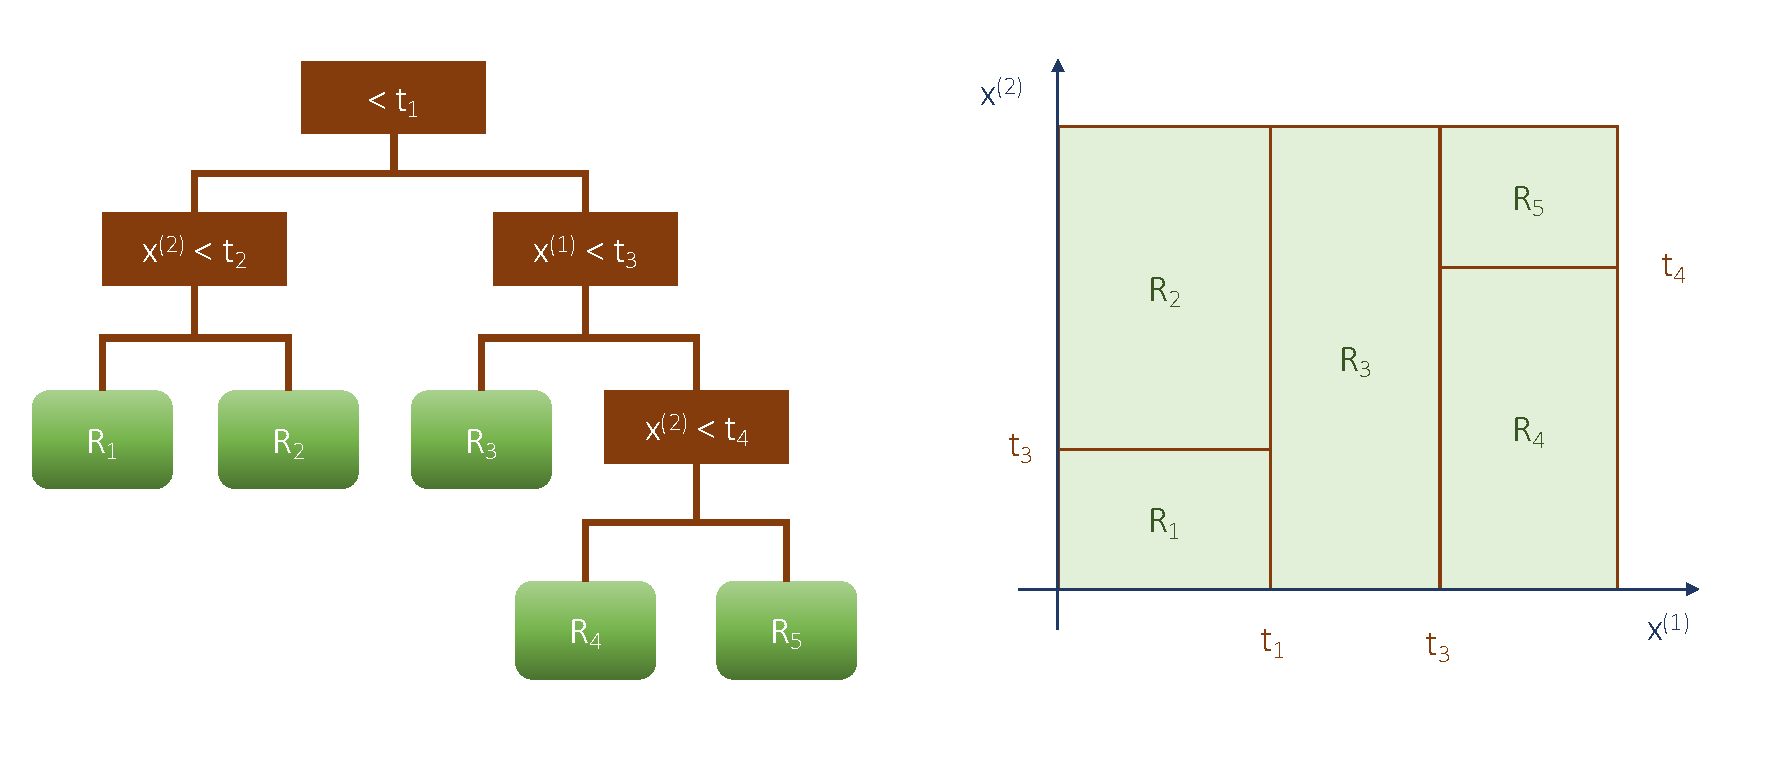
\includegraphics[width=0.8\textwidth]{figures/4-ml/decision_tree.pdf}
  \caption{Illustration of the decision tree and the region splitting performed by a CART\autocite{Breiman_2017} algorithm. Adapted from an illustration of the book ``Elements of Statistical Leanrning''~\cite{Hastie_2009}.}\label{fgr:tree}
\end{figure}

The CART\autocite{Breiman_2017} algorithm, developed by Breiman et al., is commonly presented as the archetype of a decision tree model. The algorithm follows a straightforward three-step process: (i) Examine every possible split on each feature $C_i$, (ii) select and use the best split according to a loss function (squared error or absolute error usually), and (iii) stop splitting a node when a stopping rule is satisfied (e.g.\ minimum samples split).\autocite{Dension_1998} While it is possible to split the decision tree indefinitely, assigning each data point to its own region, this would inevitably lead to a textbook case of overfitting, rendering the model incapable of accurately predicting new data points. To prevent this, the decision tree incorporates a regularization parameter known as the minimum samples split, denoted as $n\e{min}$, which restricts further splitting if a node contains fewer samples than $n\e{min}$, hence treating the latter as terminal nodes. As decision trees are very prone to overfitting, an additional useful regularization parameter, maximum depth of the tree, can be used to halt the iterative tree growth. Finally, a process known as tree pruning can be employed to further regularize decision. Tree pruning simplifies the tree structure and outputs of the final model. A comprehensive discussion of tree pruning is beyond the scope of this work (see Ref.~\cite{Hastie_2009} for further details). The final tree $f\e{tree}$ can be expressed as a function of the different regions $R_1,\ldots,R_M$ created through the splitting process:
\begin{equation}
  f\e{tree}(\mathbf{x}) = \sum_{m=1}^M c_m \mathbb{1}(\mathbf{x}\in R_m)
\end{equation}
where $c_m$ represents the value of the leaf corresponding to $R_m$, and $\mathbb{1}$ is an identity function that returns $1$ if the argument is true and $0$ otherwise. The coefficients $c_m$ of this function equivalent to the average of the labeling values in the dataset $\mathcal{D}_n$ in the region $R_m$, i.e. $c_m= \underset{i\in \mathcal{D}_n}{\text{ave}}(y_i|\mathbf{x}_i\in R_m)$.
In simple terms, the tree function returns the average value of $y$ (from the dataset) in the region where $x$ (could be new data) is located. 

The main advantage of the decision tree lies in its interpretability, as defined in the book by C. Molnar~\cite{molnar2020interpretable}. This interpretability is derived from the binary decision made at the root of the decision tree --- the explanatory characteristics ($R_m$) of a predicted value, are easily discernible, and different predictions can be imagined based on the value of $\mathbf{x}$. For smaller trees, the model can even be mentally executed. However, the decision tree model has a reputation for being highly inefficient in identifying simple linear relationships, resulting in a step-like function. It exhibits limited smoothness, with minor changes in the input $x$ potentially causing significant impacts on the predicted value (typically near the boundaries between two regions). Some changes (noise) in the training data can also profoundly alter the tree's structure. The instability of a single tree poses challenges in generalizing over unseen data.\autocite{molnar2020interpretable} To address the limitations of a single decision tree, Breiman introduced bagging predictors in 1996. This approach aims to improve the accuracy of models that exhibit instability when subjected to minor changes in the learning set.\autocite{Breiman_1996} The concept of bagging predictors has laid the foundations of random forests, which will be discussed in greater detail in the subsequent subsection.

\subsubsection{Random Forest}

The random forest is built upon the notion that a collection of weak learners, known as an ensemble model, surpasses a single strong learner. This assumption relies on a proven theorem stating that the minimal error of a forest is lower than the error of a single tree (theorem 11.2.\ of Ref.~\cite{Breiman_2001}). The strength of a model depends both on the amount of information fed into it and its level of complexity. To achieve a diverse forest consisting of weaker decision trees, two concepts are introduced: bootstrap aggregating (bagging) and random column subsampling. Both methods ensure diversity in the generated trees through random selections and promote relative weakness of the trees by reducing the amount of information accessible to each tree.

The bagging method consists in generating a set ${\left\{\phi_b\right\}}_{b\in \{1,\ldots,B\}}$ of $B$ weaker learners from different bootstrap datasets ${\left\{\mathcal{D}\ex{train}_b\right\}}_{b\in \{1,\ldots,B\}}$. Each bootstrap dataset $\mathcal{D}\ex{train}_b$ is generated by randomly selecting $t$ elements of $\mathcal{D}\ex{train}$ using a sample with replacement --- It is noteworthy that each bootstrap sample has the same number of elements as $\mathcal{D}\ex{train}$, but data points may appear multiple times within it. The frequency with which a data point $(\mathbf{x}_i,y_i)$ appears represents its weight in the bootstrap learning set. In simple terms, each tree model $\phi_b$ is trained on the $\mathcal{D}\ex{train}_b$ dataset, which assigns random weights to the data points. Therefore, each model focuses on different parts of the training data. The generalization error of the model can be evaluated, as certain trees have never seen some data points. The generalization error on unseen data for each tree (similar to cross-validation), known as the out-of-bag error, can thus be assessed. 

The second technique consists in randomly choosing a subsample of features for determining the best split (second part of the CART tree growing algorithm). This technique draws inspiration from the work of Ho in 1998, where each tree of a forest is trained exclusively on a randomly chosen subspace of feature.\autocite{Tin_Kam_Ho_1998} The only difference in the procedure lies in the fact that the feature space changes at each iteration of the tree growing process, rather than between each tree generation. This method also improves the generalizability of the approach by reducing the likelihood of overfitting in each tree, while the overall accuracy is achieved through the aggregation of all the trees.

The random forest, as formulated by Breiman, combines these two randomness-based techniques to train a forest.\autocite{Breiman_2001} The algorithm proceeds by looping over the number of trees $B$ in the forest. For each tree, denoted as $b$, a bootstrap sample $\mathcal{D}\ex{train}_b$ is randomly drawn (with replacement), and this dataset is utilized to grow the tree (training procedure). During training, a modified CART algorithm is applied to expand the tree by recursively splitting each node: (i) instead of testing all features for the best split, only a random selection of $m$ variables is considered among the $p$ features, (ii) the best split point is determined among the $m$ variables, and (iii) the node is split into two until the minimum leaf size, denoted as $n\e{min}$, is reached. The size of the column subsample defines the number of features randomly considered at each split, serving as another implicit regularization parameter associated with the random forest along with the previously identified regularization parameters of the decision tree, such as the minimal leaf size $n\e{min}$ or the maximal depth of a tree. Finally, a set of $B$ trees, denoted as $\left\{\phi_b\right\}$, is obtained, which can be used to build an ensemble model $\Phi$, such that:
\begin{equation}
  \Phi(\mathbf{x}) = \frac{1}{B}\sum_{b=1}^{B} \phi_b(\mathbf{x}) = \frac{1}{B}\sum_{b=1}^{B}\sum_{m=1}^{M_b} c_{m,b} \mathbb{1}(\mathbf{x}\in R_{m,b})
\end{equation}
It should be noted that each tree has an equal influence on the prediction, and they are trained on different random samples of the initial training data. Random forest is less prone to overfitting due to the implementation of a cross-validation process known as bootstrapping. However, the algorithm itself does not significantly improve the model's accuracy (bias error). Instead, it relies on the idea that trees mutually compensate for their individual weaknesses in the final ensemble model. In the subsequent section, an alternative algorithm will be introduced, which focuses on leveraging prior knowledge from previous trees to enhance the performance of each tree. This novel technique is referred to as boosting.

\subsubsection{From boosting to gradient boosting}\label{sct:boosting}

In the previous approach, the bootstrap dataset consists of a random selection of samples from the training set $\mathcal{D}\ex{train}$ and each tree has an equal voting weight in the final ensemble decision. However, in a boosting algorithm,\autocite{drucker1997improving} the paradigm shifts. The data samples are (i) selected based on their predictions by the previous trees, focusing on poorly predicted sample points, and (ii) the tree $\phi_b$, trained on this weighted dataset $\mathcal{D}\ex{train}_b=\left\{\left(w_i^{(b)},\mathbf{x}_i,y_i\right)\right\}$, is evaluated using a confidence $\alpha_b$, which is determined by the error made (the higher the error is, the lower the confidence is). This confidence measure is used to define the ensemble model:
\begin{equation}
  \Phi_B = \frac{1}{\sum_{b=1}^{B} \alpha_b}\sum_{b=1}^{B} \alpha_b\phi_b
\end{equation}

To train each individual tree $\phi_b$ of this forest, the CART algorithm (described in the previous sections) is utilized, but with a focus on minimizing a weighted risk function rather than the standard one:
\begin{equation}
  \mathcal{R}(\phi_b) = \sum_{i=1}^N w_i^{(b)} \mathcal{L}\left(\phi_b(\mathbf{x}_i),y_i\right)
\end{equation}
where $w_i^{(b)}$ is the normalized weight associated with the error $\mathcal{L}\left(\Phi_{b-1}(\mathbf{x}_i),y_i\right)$ made by the previous ensemble $\Phi_{b-1}$ on each data point $\left(\mathbf{x}_i,y_i\right)$. For $b=1$, when there is no previous model, the weights are equidistributed across the samples, i.e. $\forall i,\ w_i^{(1)}=1/N$. In practical applications, to simulate the weighting process, a random selection is performed on each sample with a probability $w_i^{(b)}$ to draw an equally-sized $N$ training dataset $\mathcal{D}\ex{train}_b$ for $\phi_b$. 

The specific details of the confidence rate $\alpha_b$ have not been elaborated upon intentionally, as various implementations exist. Generally, it is a decreasing function of the total error of the tree on the weighted dataset. The AdaBoost algorithm typically uses the half of the opposite of the logit transform function $\alpha_b=0.5\log\left((1-\mathcal{R}(\phi_b))/\mathcal{R}(\phi_b)\right)$, which approaches $+\infty$ for very small errors and $-\infty$ for very large ones.\autocite{Freund_1997,schapire2013explaining} Gentle AdaBoost, on the other hand, assigns an equal say to each tree independent of its performance, which, in some cases, yields better generalization performance compared to regular AdaBoost. However, very high values of $\alpha_b$ can lead to overfitting of the model in some cases, as a very good performance on the weighted dataset may indicate a good fit on noisy data points.\autocite{schapire1998improved} To prevent overfitting, an early stopping procedure with a cross-validation (typically k-fold) training procedure is performed to determine the optimal number of trees required to remain generalizable while reducing bias error. As is often the case in machine learning, this involves a trade-off between bias and variance.

In its original implementation, AdaBoost uses stamps, which are trees composed of a single splitting node and two leaves. However, boosting algorithms can be applied to trees of any depth. The tree-depth hyperparameter plays a crucial role in tree-based models as it defines the complexity/strength of each learner tree. Smaller trees generally exhibit less overfitting (see the relationship between complexity and variance in Figure~\ref{fgr:bias_variance}), and the AdaBoost algorithm uses the smallest possible tree to compensate for its highly aggressive learning procedure. The key takeaway from this study is that boosting focuses on the training trees that compensate for the errors of previous trees, and it can manipulate tree-based hyperparameters (e.g.\ tree depth, number of trees) to control variance error.

In fact, boosting can be reformulated as a gradient descent problem, as demonstrated by Mason et al.\autocite{mason1999boosting} AdaBoost can be viewed as a gradient boosting algorithm with an exponential loss function (same loss and derivative) and follows the steepest gradient descent logic.\autocite{mason1999boosting,azencott2022introduction} 

Each additional tree $\phi_{b}$ in a gradient boosting can be interpreted as a contribution to a predictor $\Phi_{b}$, leading to the minimization of an objective function $\mathcal{R}(\Phi_{b})$. The weight $w_i^{(b)}$, which measures the prediction error for each sample $i$, can be expressed as a derivative of a differentiable loss function $\mathcal{L}$ since the minimum is reached when the derivative is zero. 
\begin{equation}
  w_i^{(b)} = -\left.\frac{\partial\mathcal{L}\left(y_i,\hat{y}_i\right)}{\partial\hat{y}_i}\right|_{\hat{y}_i=\Phi_{b-1}(\mathbf{x}_i)}
\end{equation}
where $\hat{y}_i$ is a derivation variable describing the ensemble tree prediction and is evaluated at $\Phi_{b-1}$. Instead of predicting the $y_i$ values, the weight or pseudo-residual $w_i^{(b)}$ can be predicted, which measures the deviation of the previous model $\Phi_{b-1}$ from the ideal $\Phi$ (zero weights everywhere in an ideal world). This weight is compensated using a tree $\phi_{b}$. In other words, the CART framework is employed to grow a tree $\phi_{b}$ that predicts the gradients $w_i^{(b)}$ from the features $\mathbf{x}_i$, iteratively improving the model $\Phi_b$ compared to $\Phi_{b-1}$: 
\begin{equation}
  \Phi_b = \Phi_{b-1} + \eta \phi_{b}
\end{equation}
where $\eta$ is the learning rate or shrinkage, as introduced by Friedman in stochastic gradient boosting, to slow down the learning process and mitigate overfitting.\autocite{Friedman2002} In a steepest descent step, the values of this learning rate $\eta$ minimize the risk function $\mathcal{R}(\Phi_{b-1} + \eta \phi_{b})$ associated with the output model $\Phi_b$. If $b=1$, the first estimator $\Phi_1$ is simply a constant function that minimizes the risk over the training set $\Phi_1(\mathbf{x}) = \underset{c\in \mathbb{R}}{\text{arg min}} \sum_{i=1}^{N}\mathcal{L}(y_i,c)$. For a quadratic loss function, this constant corresponds simply to the average of the $y_i$ values over the training set.

In the particular case of a quadratic loss $\mathcal{L}\e{SE} =\tfrac{1}{2} {\left(y_i - f(\mathbf{x}_i)\right)}^2$ that is used in this chapter, the gradient boosting algorithm can be simply broken down into the three steps below:\autocite{Friedman2002}
\begin{enumerate}
  \item Initialization at $b=1$ with a constant: \\
    \quad $\Phi_1(\mathbf{x}) = \frac{1}{N}\sum_{i=1}^{N}y_i$
  \item For $b = 2$ to $B$:
    \begin{enumerate}
      \item Compute the pseudo-residuals, which are equivalent to real residuals in the case of a quadratic loss
        \quad $\forall i\in \{1,\ldots,N\},\ w_i^{(b)} = y_i - \Phi_{b-1}(\mathbf{x}_i)$
      \item Train the weak tree $\phi_b$ on the dataset ${\left\{ (\mathbf{x}_i, w_i) \right\}}_{i\in \{1,\ldots,N\}}$.
      \item Update the model using a fixed learning rate $\eta\in [0,1]$ instead of finding $\eta =\underset{c\in \mathbb{R}}{\text{arg min}} \sum_{i=1}^{N}\mathcal{L}\left(y_i,\Phi_{b-1}(\mathbf{x}_i) + c \phi_b(\mathbf{x}_i)\right)$ through a minimization problem (steepest gradient descent).
        \quad $\Phi_b = \Phi_{b-1} + \eta \phi_{b}$
    \end{enumerate}
  \item Output the final ensemble model $\Phi_B$
\end{enumerate}

Up until now, the different ways of utilizing decision trees to perform predictions on a training dataset $\mathcal{D}\ex{train}$ have been demonstrated, with a specific focus on two ensemble models: random forest and gradient boosted trees. The aim of exploring these models is to introduce a prediction model that combines techniques from both ensemble models. This model, known as eXtreme Gradient Boost or XGBoost, was introduced by Chen et al.\ and offers improved scalability compared to similar methodologies. The implementation improvements will not be discussed in detail here (see Ref.~\cite{chen2016xgboost} for more details). Instead, the focus will be on the fundamental framework employed by XGBoost, which will enable a better understanding of its core components.

\subsubsection{XGBoost model parameterization}

The XGBoost model essentially constitutes a gradient boosting model, as discussed in the previous section, with several regularization parameters that can be fine-tuned to enhance its generalizability. In a learning problem involving $N$ learning examples and $p$ features/descriptors, the predictor $\Phi$ can be expressed as the sum of weaker tree learners $\phi_b$:
\begin{equation}
  \Phi(\mathbf{x}) = \sum_{b=1}^{B} \phi_b(\mathbf{x}) = \sum_{b=1}^{B} \sum_{m=1}^{M}c_m^{(b)} \mathbb{1}(\mathbf{x}\in R_m^{(b)})
\end{equation}
where $M$ is the maximal number of leaves a tree can have, in our implementation --- this number is fixed using the maximum depth $\max\e{depth}$ in the algorithm since $M=2^{\max\e{depth}}$, and $B$ is the maximum number of estimators in the ensemble model. The number of estimators is typically determined using early stopping in k-fold cross-validation. 

A quadratic loss function, with L1 and L2-regularization terms, was applied to the $M$ leaf weights $c_m$ of a model $phi$, resulting in the following expression for the loss function $\mathcal{L}$: 
\begin{equation}
  \mathcal{L}\left(y,\phi(\mathbf{x}_i)\right) = \tfrac{1}{2}{\left(y - \phi(\mathbf{x}_i)\right)}^2 + \lambda_1 \sum_{m=1}^{M}\left\lvert{c_m^{(b)}}\right\rvert + \lambda_2 \sum_{m=1}^{M}{\left\lvert{c_m^{(b)}}\right\rvert}^2 
\end{equation}
where $\lambda_1$ and $\lambda_2$ are the L1 and L2-regularization coefficients that control the importance of each regularization term. 

The risk function $\mathcal{R}$ of a tree $\phi_b$ with $M$ leaf weights $c_m^{(b)}$ at the iteration $b$ of the gradient boosting process can be expressed as follows:
\begin{equation}
  \mathcal{R}(\phi_b) = \frac{1}{N}\sum_{i=1}^{N} \tfrac{1}{2}{\left(w_i^{(b)} - \phi_b(\mathbf{x}_i)\right)}^2 + \lambda_1 \sum_{m=1}^{M}\left\lvert{c_m^{(b)}}\right\rvert + \lambda_2 \sum_{m=1}^{M}{\left\lvert{c_m^{(b)}}\right\rvert}^2 
\end{equation}
where $w_i^{(b)}$ is the pseudo-residuals of the previous model on the dataset. This expression of the risk is typically used in the tree-splitting process of the step 2.(b) of the gradient boosting algorithm (see previous subsection~\ref{sct:boosting}) to find the best tree that will be used to predict the pseudo-residuals. As explained earlier, the pseudo-residual is defined as the difference between the observed value $y_i$ and the previously predicted value $\Phi_{b-1}(\mathbf{x}_i)$, also known as the residual in regression problems, in the case of a quadratic loss:
\begin{equation}
  w_i^{(b)} = -\left.\frac{\partial\mathcal{L}\left(y_i,\hat{y}_i\right)}{\partial\hat{y}_i}\right|_{\hat{y}_i=\Phi_{b-1}(\mathbf{x}_i)} = y_i - \Phi_{b-1}(\mathbf{x}_i)
\end{equation}

The learning rate $\eta$ used for updating the ensemble model is also a key component of the final model that needs to be adjusted to maximize the generalizability of the model. This parameter slows down and smoothens the convergence to the solution, thereby improving the bias--variance trade-off. Small values below $0.1$ are typically used.

\begin{table}[ht]
  \setlength{\extrarowheight}{1pt}
  \centering
  \begin{tabular}{|l|c|m{8cm}|}
  \hline
    Variable name  &  Variable   &   Description\\
    in XGBoost  &    in this work &  of the hyperparameter \\
  \hline
      "n\_estimators" &   $M$ &   Number of trees in the final ensemble model  \\
      "max\_depth" &      $\simeq\log_2(T)$ &   Maximum number of levels allowed for each tree that can be expressed as a function of $T$ the number of terminal nodes or leaves \\
      "alpha" &   $\lambda_1$ &   L1-regularization parameter  \\
      "lambda" &   $\lambda_2$ &  L2-regularization parameter  \\
      "learning\_rate" &   $\eta$ &   The shrinkage or learning rate used to update the ensemble model with each basic tree.  \\
      "subsample" &   $N\e{sample}/N$ &   The ratio of data points randomly sampled (without replacement) for the training of each tree $\phi_b$  \\
      "colsample\_bytree" &   $p\e{tree}/p$  &   The ratio of features randomly sampled per tree iteration (on $b=1$ to $B$)  \\
      "colsample\_bylevel" &   $p\e{level}/p$  &   The ratio of features randomly sampled per level iteration (on $k=1$ to $M$, this would be on the leaves really but to simplify) \\
  \hline
  \end{tabular}
  \caption{Hyperparameters of XGBoost relevant to our work.}\label{tab:hyperparameter}
\end{table}

To add randomness in the gradient descent procedure, three other parameters that are very similar to the ones implemented in a random forest were utilized. With the integration of these techniques, the model can be referred to as stochastic gradient boosting, as described in the Ref.~\cite{Friedman2002}. In each iteration, a random subsample of the training data is drawn (without replacement) based on a parameter $N\e{sample}/N$. This parameter has a similar effect as the bagging procedure of the random forest, restricting the focus of each weak learner to a portion of the learning set. This approach reduces overfitting, akin to a cross-validation procedure. The different trees learn from distinct segments of the training set, preventing the ensemble model from overfitting the entire dataset. This provides an effective solution to the well-known issue of overfitting encountered in standard gradient boosting. Another procedure involves randomly selecting feature columns, inspired by the concept introduced in Ref.~\cite{Tin_Kam_Ho_1998}. It entails randomly extracting a subsample of the features for the training of each tree. A parameter is required to determine the size of the portion of features  $p\e{tree}/p$ used for training each tree. Similarly, column sampling can be performed at each level rather than for each tree, where a proportion $p\e{level}/p$ is defined accordingly. Alternatively, a random feature sampling at the node level is also a plausible option, although this parameter was not utilized in this context.

Finally, the parameters used in the construction of the final model are compiled in Table~\ref{tab:hyperparameter}. The table encompasses a tree-specific parameter "max\_depth", an ensemble-specific parameter, "n\_estimators", general regularization parameters inspired by linear models "alpha" and "lambda", along with a more gradient boosting specific parameter "learning\_rate", and more randomness-based hyperparameters inspired by random forest, such as "subsample", "colsample\_bytree" and "colsample\_bylevel". This model can be considered as a blending of various concepts drawn from diverse domains within the field of data science. By using this machine learning model, the selectivity drop problem discussed in the preceding chapter will be addressed.

\section{Prediction of the ambient-pressure selectivity}

Before delving into the model of this work, the different literature contributions to xenon/krypton separation screenings will be briefly reviewed. Simon et al.\ published one of the first articles on an ML-assisted screening approach for the separation of a Xe/Kr mixture extracted from the atmosphere.\autocite{Simon_2015} Their model's performance heavily relied on the Voronoi energy, which represents an average of the interaction energies of a xenon atom at each Voronoi node.\autocite{Rycroft_2009} To rationalize this increase in performance, the Voronoi energy can be considered as a faster proxy for the adsorption enthalpy. A comparison with the standard Widom insertion revealed that, although faster, the Voronoi energy is less accurate. To address this, a more effective alternative called surface sampling (RAESS) was developed, utilizing symmetry and non-accessible volumes blocking (see section~\ref{sct:RAESS}). Recently, Shi et al.\ used an energy grid to generate energy histograms as a descriptor for their ML model. This approach provides an exhaustive description of the infinitely diluted adsorption energies\autocite{Shi_2023} but can be computationally expensive.

While the aforementioned approaches demonstrate good accuracy in predicting low-pressure adsorption (i.e., in the limit of zero loading), they are not suitable for predicting adsorption in the high-pressure regime when the material is near saturation uptake. Grand Canonical Monte Carlo (GCMC) simulations are commonly employed for this task, but there is a lack of methods for decreasing computational costs for high-throughput screening. The challenge this thesis aims to address is predicting selectivity in the nanopores of a material at high pressure, where adsorbates interact with each other, while having access to information only on the interaction at infinite dilution. Comparing the low- and high-pressure cases provides key information on the origin of selectivity differences. Previous studies have shown that selectivity can decrease between the low and ambient pressure cases in Xe/Kr separation applications (see chapters 2 and 3), primarily due to the presence of different pore sizes and potential reorganizations caused by adsorbate--adsorbate interactions.

By combining grid-based descriptors described in the previous chapter (section~\ref{sct:grid}) with statistical characterizations of pore size, a set of ML descriptors suitable for rapid and accurate ambient-pressure selectivity prediction was proposed. These descriptors were used in an optimized XGBoost model, showcasing its performance in the case of xenon/krypton separation in the CoRE MOF 2019 database\autocite{Chung_2019}. The study presented in the following is in the process of being published, and a preprint is avaible on \emph{Chem. rXiv} in Ref.~\cite{Ren_2023_ml}.\footnote[1]{The corresponding data and scripts can be found at: \url{} \todo{create a repo github with the different models and data}}

\subsection{Data Preparation}


\subsubsection{Target variable}

This study aims at building an ML model to predict the Xe/Kr ambient-pressure selectivity faster than standard techniques. To obtain reference values (ground truth), I used the RASPA2 software\autocite{dubbeldam2016} to run GCMC calculations (introduced in section~\ref{sct:GCMC}) of 20–80 Xe/Kr mixtures at \SI{298}{\kelvin} and \SI{1}{\atm} on our cleaned database. The van der Waals interactions are described by a Lennard-Jones (LJ) potential with a cutoff distance of \SI{12}{\angstrom}. The LJ parameters of the framework atoms are given by the universal forcefield (UFF),\autocite{rappe1992} and the guest atoms (xenon and krypton) have their LJ parameters taken from a previous screening study.\autocite{Ryan_2010} The study only focuses on a given Xe/Kr composition usually obtained by cryogenic distillation of ambient air~\autocite{kerry2007industrial} as a first step towards predicting other mixtures at different physical conditions (\emph{e.g.} Xe/Kr mixtures out of nuclear off-gases). 

To achieve this, a logarithmic transform of the selectivity will be considered instead of the raw value because the goal is rather to predict the order of magnitude of the selectivity values than to predict the higher values of selectivity --- an ML model that focuses its prediction on raw selectivity values can reach lower errors by simply focusing on the higher values than the lower ones. By focusing on the logarithmic transform of the selectivity, the different selectivity categories can be separated through the different orders of magnitude of the selectivity values. This approach distributes more evenly the efforts on all the whole spectrum of selectivity values. Moreover, this logarithmic transformation is effectively an exchange Gibbs free energy that was introduced in chapter 2 and redefined in equation~\ref{eq:exc_gibbs}; it can therefore be easily compared with the energy descriptors I introduced in the previous chapter 3.
\begin{equation}\label{eq:exc_gibbs}
  \Delta\e{exc}G = -RT \ln\left(s\right)
\end{equation}

\subsubsection{Database and data generation}

This methodology is tested on a set of realistic MOFs by considering the 12\,020 all-solvent removed (ASR) structures of the CoRE MOF 2019 database\autocite{Chung_2019}. After removing the disordered and the non-MOF structures as well as the ones with a large unit cell volume of \SI{20}{\cubic\nano\meter}, the database is reduced to a set of 9,748 structures. Then, with the string information given by the Zeo++ software\autocite{zeopp_Willems2012} this number is reduced to 9\,177 by removing the structures that are not tridimensional, where solvents are still detected (wrongly classified in ``all solvent removed''), or where the metal is radioactive or fissile (e.g., Pu-MOF \texttt{TAGCIP}\autocite{Diwu_2010}, Np-MOF \texttt{KASHUK}\autocite{Martin_2017}, U-MOF \texttt{ABETAE}\autocite{Jouffret_2011} or Th-MOF \texttt{ASAMUE}\autocite{Liang_2016}) --- this can be a source of risks in a nuclear waste processing plant. Furthermore, a condition on the largest cavity diameter (LCD) is added to keep only the structures with pore sizes allowing the adsorption of xenon: this is the case for 8\,529 structures with an LCD higher than \SI{4}{\angstrom} (approximately the size of a xenon molecule). This is equivalent to removing the structures with very unfavorable adsorption enthalpies, that are not promising for our adsorption-based separation.

Then, the descriptors summarized below (and fully detailed in Supporting Information) were calculated on this restrained dataset. At this stage, 370 structures failed to be calculated in GCMC\todo{change} and 82 have a zero value for the standard deviation of the pore distribution (skewness and kurtosis go to infinite and cannot be defined). A final dataset of 8,077 structures was therefore used to perform our ML-assisted method of screening the Xe/Kr adsorption selectivity. Based on this final set, {20\%} were randomly used for the test set and {80\%} were used to train our model. The goal is to learn from the training set a relationship between the descriptors and the target ambient-pressure selectivity in order to evaluate the performance on the test set. A CSV file of training and test sets can be found in the data availability section.

\subsection{Feature engineering}

\subsubsection{Geometrical and chemical ML descriptors}

Examining a number of research papers on supervised ML for the prediction of adsorption properties,\autocite{Fernandez_2013,Simon_2015,Fanourgakis_2020,Anderson_2020,Pardakhti_2020} recurrent descriptors are identified: (i) geometrical descriptors obtained using software like Zeo++~\autocite{zeopp_Willems2012} including surface area (SA), void fraction (VF), largest cavity diameter (LCD) and pore limiting diameter (PLD); and (ii) physical and chemical descriptors such as framework density, framework molar mass, percentage of carbon (C\%), nitrogen (N\%), oxygen (O\%), hydrogen, as well as halogen, nonmetals, metalloids and metals, and degree of unsaturation. Although these descriptors are versatile and widely used in ML models, they fail to provide specific information for the ML task of this study. As demonstrated by Simon et al., energy descriptors greatly influence ML models for selectivity prediction.

The geometric analysis of crystalline porous materials is typically based on the predefined van der Waals (vdW) radii from the Cambridge Crystallographic Data Centre (CCDC). This forcefield-independent choice can create a gap between geometrical descriptors and thermodynamic values obtained through molecular simulations. Inspired by a recent work comparing PLDs and self-diffusion coefficients,\autocite{Hung_2021} a list of vdW radii was defined to be read by the Zeo++ software (more details can be found at \url{github.com/eren125/zeopp_radtable}). In this study, all Zeo++ calculations utilize an atomic radius that corresponds to the distance at which the LJ potential reaches $3 k_\text{B} T/2$ at $T = \SI{298}{\kelvin}$.

The SA exposed to different probe sizes (\SI{1.2}{\angstrom}, \SI{1.8}{\angstrom} and \SI{2.0}{\angstrom}) was tested. The probe occupiable volume was chosen to measure the void fraction (VF) for different adsorbent using probe sizes of \SI{1.8}{\angstrom} (close to the radius of krypton) and \SI{2.0}{\angstrom} (close to that of xenon). This definition of pore volume demonstrated better agreement with experimental nitrogen isotherms.\autocite{vol_Ongari2017}

Given the objective of predicting the difference between low-pressure selectivity and ambient-pressure selectivity (for a specific gas mixture composition), some descriptors hold little importance, and the key factor lies in the difference in accessible volume and affinity of the remaining pore volume with xenon compared to krypton. The intuition developed in chapter 2 outlines the role of a diverse distribution of pores with different xenon affinities. Therefore, from the ``standard'' descriptors mentioned in the literature, the following 7 descriptors were retained: C\%, N\%, O\%, LCD ("D\_i\_vdw\_uff298"), PLD ("D\_f\_vdw\_uff298"), SA for a \SI{1.2}{\angstrom} probe ("ASA\_m2/cm3\_1.2") and VF for a \SI{2.0}{\angstrom} probe ("PO\_VF\_2.0"). Additionally, a new descriptor $\Delta \text{VF}$ was created to represent the difference in void fraction values, specifically the difference in volumes occupiable by xenon (\SI{2.0}{\angstrom}) and krypton (\SI{1.8}{\angstrom}). A comprehensive presentation of all these descriptors, including other geometrical descriptors based on pore size distribution, can be found in Table~S1 of the Supplementary Information (SI).

\subsubsection{Pore size statistics}

To generate a histogram of pore sizes (or pore size distribution, PSD), Monte Carlo steps are used to measure the frequency of every accessible pore sizes binned by \SI{0.1}{\angstrom}.\autocite{poresize_Pinheiro2013} This histogram can then be utilized to generate descriptors based on statistical parameters that describe the overall location, dispersion, shape, and modality of the distribution. In addition to the mean and standard deviation of the distribution, two additional moments were introduced: the skewness ($\gamma$), which corresponds to the third standardized moment and measures the asymmetry of a distribution; and the kurtosis ($k$), being the fourth standardized moment, measures the relative weight of the distribution's tails. Recognizing the importance of characterizing the number of different pore sizes that are likely to have contributed to the observed selectivity drop, this study tried find a simple descriptor for measuring the number of modes in the distribution. The Sarle's bimodality coefficient, BC $= (\gamma^2 +1)/k$, provides a simple quantification of the extent to which the distribution deviates from unimodality by considering only skewness and kurtosis\autocite{Tarba_2022}.

Finally, to assess the diversity of pores, an effective number $n\e{eff} = N^2/\sum n_i^2$ of pore sizes was introduced, where $N$ represents the total number of points in the histogram and $n_i$ the number of points associated with the $i^\text{th}$ bin. This number bears resemblance to a statistical measure widely used in other scientific domains. In political science, it is employed to measure the effective number of political parties,~\autocite{neffposci_Laakso1979} while in ecology, the inverse Simpson's index evaluates the species diversity in an ecosystem,\autocite{neffbio_Simpson1949}. Similarly, in quantum physics, the inverse participation number measures the degree of localization of a wave-function.\autocite{neffphys_Kramer1993} This effective number of pore sizes provides an indication of the diversity of pore sizes (considering a binning of \SI{0.1}{\angstrom}). A highly effective number suggests that multiple pore sizes are well represented in the structure. Thus, this descriptor provides insight into the scattering of pore sizes within the distribution.
All these descriptors contain valuable information regarding the form of the PSD required to understand the loading and selectivity situation in the framework near saturation uptake, which is crucial to predict the ambient-pressure selectivity.

\subsubsection{Grid-based and geometrical descriptors}

The low-pressure selectivity provides a first intuition about the selectivity at higher pressure, as demonstrated in the previous work, where a correlation between selectivity at both pressures (section~\ref{section:pressure}) was observed. If the Gibbs free energy formalism is adopted(Equation~\ref{eq:exc_gibbs_free_energy}), which correspond to a logarithmic transform of the selectivity values, this correlation is confirmed and illustrated in Figure~\ref{fgr:problem}. It is worth noting that while the selectivity of the majority of structures remains similar under both pressure conditions, a few structures experience a drop in selectivity at higher pressure. The grid sampling approach consistently yields zero-loading selectivity values that are higher or comparable to the ambient-pressure selectivity, providing a reliable foundation for the development of an efficient prediction model. The development of explanatory descriptors related to this selectivity drop phenomenon is the second requirement for a good prediction model. The presence of larger pores, which are less attractive to xenon, is one of the main causes of the selectivity drop. Therefore, additional information on the pore size distributions or the energy landscape would be helpful for this task.

\begin{figure}[ht]
\centering
  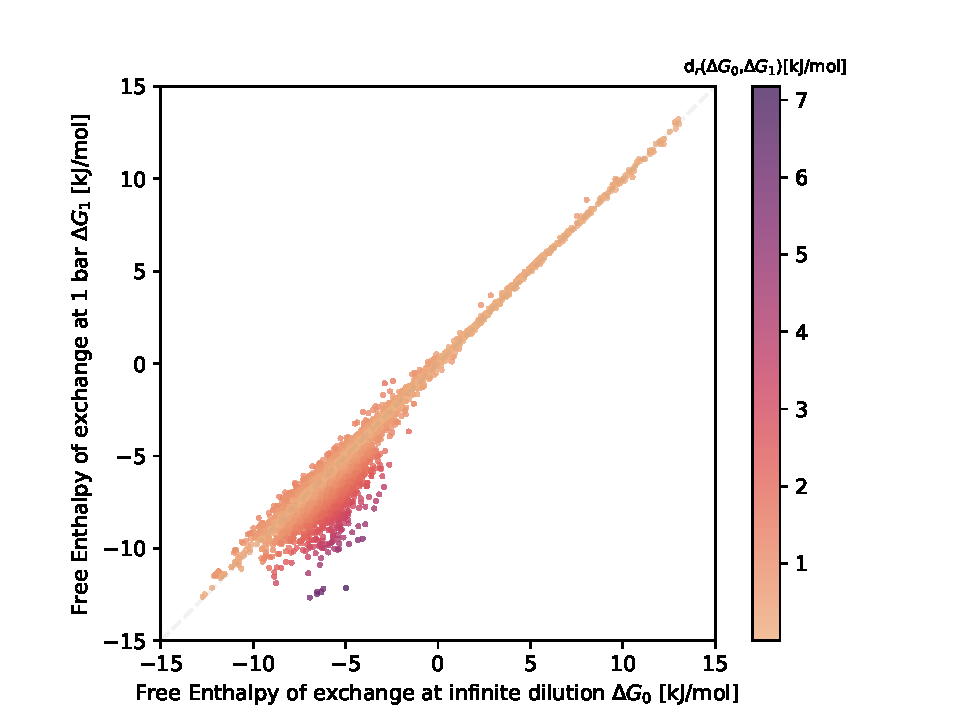
\includegraphics[width=0.5\linewidth]{figures/4-ml/main/Scatterplot_G1_G0.pdf}
  \caption{Comparison between the Gibbs free energy of exchange at low pressure $\Delta G\e{0}$ and ambient pressure $\Delta G\e{1}$ labeled by the relative distance between them. This plot is equivalent to a logarithmic plot of the selectivity at these two pressure conditions.}
  \label{fgr:problem}
\end{figure}

%% Pore size distribution & statistical descriptors
To incorporate information on the pore size diversity of the materials, statistical measurements were carried out on the PSD. Explanatory factors at the origin of the observed selectivity drop were detected through analysis. A high degree of multi-modality in the distribution would indicate a diverse set of pores, which can result in a selectivity drop if the pores significantly differ from each other. The chance of observing a selectivity drop increases as the average pore size deviates further from the largest cavity diameter, as a substantial difference in pore sizes leads to lower selectivity. These statistics aim to provide extensive knowledge about a hypothetical selectivity drop and quantitatively estimate its magnitude.

%% Energy descriptors statistics
To better quantify the change of selectivity, it could be interesting to present statistics on the distribution of interaction energies for xenon and krypton calculated by the grid algorithm. These statistics include moments of different orders (up to 4) of the energy distribution, which inform on the adsorbate--adsorbent interaction energies in the nanopores at higher loading. 
Analyzing the shape of the energy distribution facilitates a quantitative assessment of the selectivity change. This approach compresses the entire energy distribution into a few statistical values, a common method employed in data science to tackle distribution data. The same methodology has been applied to Boltzmann weighted distributions to generate temperature-specific descriptors for the energy distributions. All these quantities have been calculated and compared to ambient-pressure selectivity in the previous chapter (section~\ref{sct:grid}).

%% 900K gaps
As explained in the previous chapter, Boltzmann averaging at higher temperature provided better results in describing ambient-pressure selectivity. 
This novel type of descriptor proves particularly effective in the high selectivity region, where the standard Boltzmann average at \SI{298}{\kelvin} loses its accuracy (Figure~\ref{fgr:H_900K}). This descriptor was utilized to build several descriptors presented in Table~\ref{tab:energy_descriptors}. As illustrated in Figure~\ref{fgr:featimp_shap}, the exchange Gibbs free energy at \SI{900}{\kelvin} and the excess of free energy compared to the \SI{298}{\kelvin} case rank as the second and third most influential descriptors in this ML model. They complement the exchange Gibbs free energy at \SI{298}{\kelvin} in predicting selectivity at higher pressures.

%% conclusion
By combining the above-mentioned features with more standard geometrical descriptors, an ML model was trained for ambient pressure selectivity. The model identifies the origins of the selectivity drop and yields promising prediction results.

\clearpage

\begin{table}[ht]
  \setlength{\extrarowheight}{1pt}
  \centering
  \begin{tabular}{|l|m{10cm}|}
  \hline
   {Feature name} &  {Description} \\
  \hline
  "ASA\_m2/cm3\_1.2"  & Volumetric surface area accessible to a nitrogen probe (\SI{1.2}{\angstrom}) in \si{\square\meter\per\cubic\centi\meter} \\
  \hline
  "delta\_VF\_18\_20"  & Difference of void fraction occupiable by a krypton (\SI{1.8}{\angstrom} radius) and a xenon  (\SI{2.0}{\angstrom} radius) probe. Always positive due to the difference of probe radii. \\
  \hline
  "PO\_VF\_2.0"  & Void fraction occupiable by a xenon probe of  \SI{2.0}{\angstrom} radius \\
  \hline
  "D\_i\_vdw\_uff298"  & Largest cavity or largest included sphere diameter (LCD). Structures atom radii are defined using the UFF forcefield\textsuperscript{1} \\
  \hline
  "D\_f\_vdw\_uff298"  & Pore Limiting Diameter (PLD) or largest free sphere diameter defined similarly to the LCD  \\
  \hline
  "pore\_dist\_mean"  & Mean value of the pore size distribution or the average pore size \\
  \hline
  "delta\_pore"  & Difference between the LCD and the average pore size: "delta\_pore" $=$ "D\_i\_vdw\_uff298" $-$ "pore\_dist\_mean" \\
  \hline
  "pore\_dist\_std"  & Standard deviation of the pore size distribution \\
  \hline
  "pore\_dist\_skewness"  & Skewness (third order standardized moment) of the pore size distribution  \\
  \hline
  "pore\_dist\_kurtosis"  & Kurtosis (fourth order standardized moment) of the pore size distribution \\
  \hline
  "pore\_dist\_neff"  & Effective number of data associated to the pore size distribution: $N\e{eff} =$ sum(weights)$^2$ $/$ sum(weights$^2$) \\
  \hline
  "pore\_dist\_modality"  & Sarle's bimodality coefficient (BC) of the pore size distribution: BC $=$ kurtosis $-$ skewness$^2$ \\
  \hline
  "C\%"  & Percentage of carbon (C) in the MOF structure \\
  \hline
  "O\%"  & Percentage of oxygen (O) in the MOF structure  \\
  \hline
  "N\%"  & Percentage of nitrogen (N) in the MOF structure  \\
  \hline
  \end{tabular}
  \caption{Description of geometrical and chemical features used in the ML model.}\label{tab:geom_descriptors}
  \end{table}

\footnotetext[1]{Using the approach of Ref.~\cite{Hung_2021}}
\clearpage

  \begin{table}[ht]
  \centering
  \setlength{\extrarowheight}{1pt}
  \begin{tabular}{|l|m{10cm}|}
  \hline
   {Feature name} &  {Description} \\
  \hline
  "G\_0"  & Low-pressure Xe/Kr exchange Gibbs free energy defined using the low-pressure selectivity: \\
  & $\Delta\e{exc} G\ex{Xe/Kr} = -RT\ln{\left(s\ex{Xe/Kr}\right)}$ \\
  \hline
  "G\_Xe\_900K"  & High temperature Xe adsorption Gibbs free energy defined using the Henry's constant: \\
  & $\Delta\e{ads} G\ex{Xe} (T\e{h}) = -RT\e{h}\ln{\left(RT\e{h}\rho_fK\e{H}\ex{Xe}(T\e{h})\right)}$ \\
  \hline
  "G\_Kr\_900K"  & High temperature Kr adsorption Gibbs free energy: \\
  & $\Delta\e{ads} G\ex{Kr} (T\e{h})$ \\
  \hline
  "G\_900K"  & High temperature Xe/Kr exchange Gibbs free energy: \\
    & $\Delta\e{exc} G\ex{Xe/Kr} (T\e{h}) = -RT\e{h}\ln{\left(K\e{H}\ex{Xe}(T\e{h})/K\e{H}\ex{Kr}(T\e{h})\right)}$ \\
  \hline
  "delta\_G0\_298\_900"  & Difference of exchange free energies between the ambient temperature and high temperature: \\
  & $\Delta\e{T} H\ex{Xe/Kr} = \Delta\e{exc} G\ex{Xe/Kr} (T\e{h})-\Delta\e{exc} G\ex{Xe/Kr} (T\e{0})$ \\
  \hline
  "delta\_H0\_Xe\_298\_900"  & Difference of Xe adsorption enthalpy between the ambient temperature and high temperature: \\
  & $\Delta\e{T} H\ex{Xe} = \Delta\e{ads} H\ex{Xe} (T\e{h})-\Delta\e{ads} H\ex{Xe} (T\e{0})$ \\
  \hline
  "delta\_TS0\_298\_900"  & Difference of exchange entropic term between the ambient temperature and high temperature: \\
    & $\Delta\e{T} \left(-T\Delta\e{exc}S\ex{Xe/Kr}\right) = \Delta\e{T} \left(\Delta\e{exc}G\ex{Xe/Kr} - \Delta\e{exc}H\ex{Xe/Kr}\right)$ \\
  \hline
  "enthalpy\_std\_xenon"  & Standard deviation of the Boltzmann weighted Xe energy distribution \\
  \hline
  "enthalpy\_std\_krypton"  & Standard deviation of the Boltzmann weighted Kr energy distribution \\
  \hline
  "enthalpy\_skew"  & Skewness of the Boltzmann weighted Xe energy distribution \\
  \hline
  "enthalpy\_modality"  & Bimodality coefficient of the Boltzmann weighted Xe energy distribution \\
  \hline
  "mean\_grid\_xenon"  & mean value of the xenon interaction energy distribution \\
  \hline
  "mean\_grid\_krypton"  & mean value of the krypton interaction energy distribution \\
  \hline
  "std\_grid\_xenon"  & standard deviation of the xenon interaction energy distribution \\
  \hline
  "std\_grid\_krypton"  & standard deviation of the krypton interaction energy distribution \\
  \hline
  \end{tabular}
  \caption{Description of the 15 energy-based features used in the ML model. Thermodynamic descriptors are always defined at low pressure as they are derived from an interaction energy grid. Temperatures are defined as follows: T\e{0}=298~\si{\kelvin} and T\e{h}=900~\si{\kelvin}. All these energy values are defined in \si{\kilo\joule\per\mole}.}\label{tab:energy_descriptors}
  \end{table}
  
  \clearpage

\subsection{Model training}

\subsubsection{The machine learning model}

The eXtreme Gradient Boosting (XGBoost) algorithm was chosen as the machine learning framework for the predictive model due to its accuracy, efficiency, and simplicity of use. Its performance has been extensively demonstrated, as evidenced by 17 out of 29 winning solutions in Kaggle Challenges being based on this algorithm in 2015. The XGBoost system is highly scalable and parallelized, resulting in fast model training.\autocite{chen2016xgboost} Compared to more conventional tree-based algorithms like random forest (commonly used in the field~\autocite{Simon_2015}), the boosting component of the algorithm enables learning from previous mistakes and allocating greater effort to problematic data points, thereby improving the accuracy of the final ML model.

In the following sections, new descriptors for nanoporous materials will be introduced, along with novel concepts of feature engineering based on energy and pore size histograms. The ML features have been selected through progressive filtering, eliminating less influential features on the accuracy of the final model. The complete list can be found in Table S1-3 of the Supporting Information (SI). The influence or importance of these features will be defined in a subsequent section dedicated to model interpretation. The hyperparameters of the model were fine-tuned through random searches to design the best-performing final model. Lastly, a unified approach will be employed to interpret the influence of the preselected descriptors on the final model.

\subsubsection{Hyperparameter optimization}\label{sct:hyperparameter}

The search for hyperparameters involves finding the best model to optimize the generalization error, as defined in equation~\ref{eq:generalization_error}. The most common strategy is to perform cross-validations to evaluate different model configurations, known as hyperparameter search or optimization. In this case, the randomized search algorithm was utilized to find the best parameters within a predefined reasonable range. Through a random search of 30\,000 iterations on the parameter space, a set of optimal hyperparameters (refer to Table~\ref{tab:hyperparameter} for the meaning of the parameters) for the final ML model was obtained using the following Python dictionary:

\begin{lstlisting}[language=Python]
params = {
           'n_estimators': [1500],
           'max_depth': [5,6],
           'learning_rate': [0.02,0.04,0.06,0.08],
           'colsample_bytree': np.arange(0.6, 1.0, 0.05),
           'colsample_bylevel': np.arange(0.6, 1.0, 0.05),
           'alpha': np.arange(0, 4, 0.2),
           'subsample': np.arange(0.6, 0.95, 0.05),
         }
\end{lstlisting}

At each iteration, the hyperparameters of the model were evaluated using a 5-fold cross-validation on the training data. The final set of optimal hyperparameters, which corresponded to the model with the lowest RMSE of \SI{0.36}{\kilo\joule\per\mole} is provided below. This final set of parameters was then used to train the final model.

\begin{lstlisting}[language=Python]
  optimal_params = {
      'objective': 'reg:squarederror',
      'n_estimators': 1500,
      'max_depth': 6,
      'colsample_bytree': 0.85,
      'colsample_bylevel': 0.65,
      'subsample': 0.7,
      'alpha': 0.4,
      'lambda': 1,
      'learning_rate': 0.04,
      }
  \end{lstlisting}

To confirm the relevance of the model, another 5-fold cross-validation was performed using the set of parameters mentioned above. The convergence plot of the XGBoost model with this parameter set is shown in Figure~\ref{fgr:convplot}. With this configuration, the model was tested on the predefined test set, and interpretation tools were employed to gain a better understanding of the structure-property relationships at play.

\begin{figure}[ht]
  \centering
    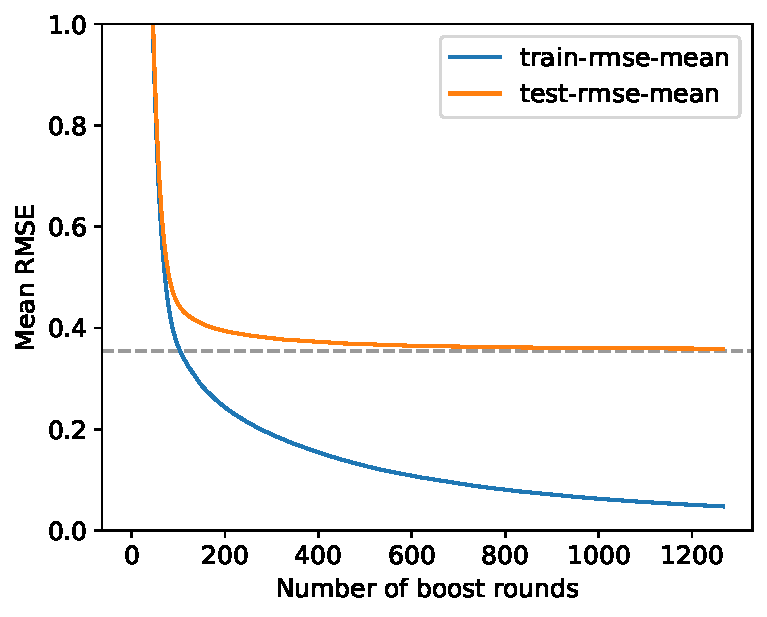
\includegraphics[width=0.60\linewidth]{figures/4-ml/SI_figure/convergence_plot.pdf}
    \caption{Convergence plot of the cross-validation training of our ML model. With the training set considered, the generalization error on the test set converges to 0.36~\si{\kilo\joule\per\mole}.}\label{fgr:convplot}
  \end{figure}

\subsection{ML model performance}

%% introduction
In this section, the performance of the ML model, which learned the joint effects of all the newly introduced descriptors, will be presented to detect and evaluate the observed drop between the easily accessible low-pressure selectivity and the more computationally demanding ambient-pressure selectivity. A GCMC simulation of a 20–80 xenon/krypton gas mixture required an average of 2 400~\si{\second} per structure on the CoRE MOF 2019 database, while the grid-based adsorption calculation only took about \SI{5}{\second} per structure (on a single Intel Xeon Platinum 8168 core at \SI{2.7}{\giga\hertz}). Computing all the necessary features for the prediction would take less than a minute per structure, significantly faster than the 40 minutes required for a GCMC calculation. The ML-based approach clearly demonstrates a speed advantage over standard molecular simulations. However, it needs to maintain a high level of accuracy on an unseen set of structures to be a good substitute.

\begin{figure}[ht]
\centering
  \begin{subfigure}[b]{0.48\textwidth}
  \centering
    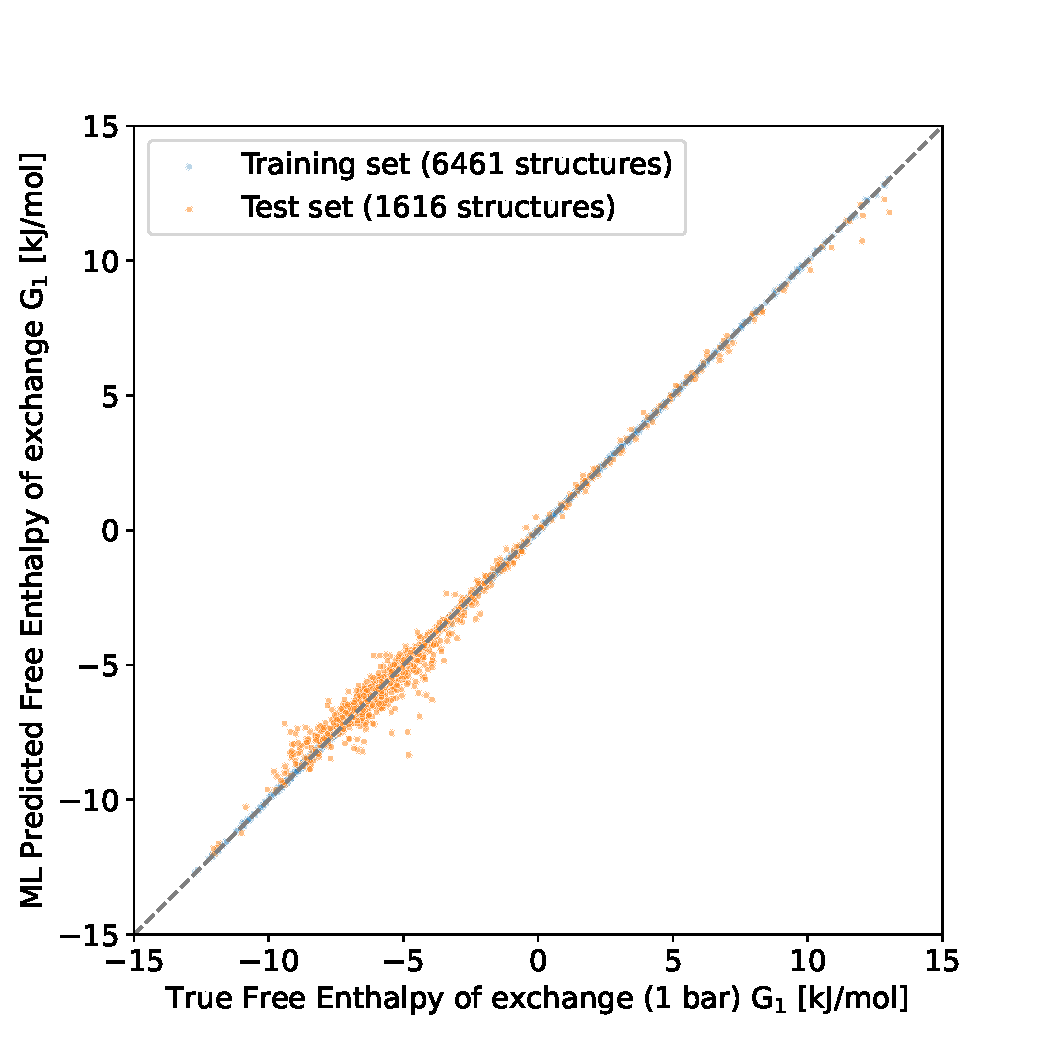
\includegraphics[width=\textwidth]{figures/4-ml/main/Scatterplot_G1_prediction.pdf}
    \caption{Final model prediction}\label{fgr:G1_prediction}
  \end{subfigure}
  \begin{subfigure}[b]{0.48\textwidth}
  \centering
    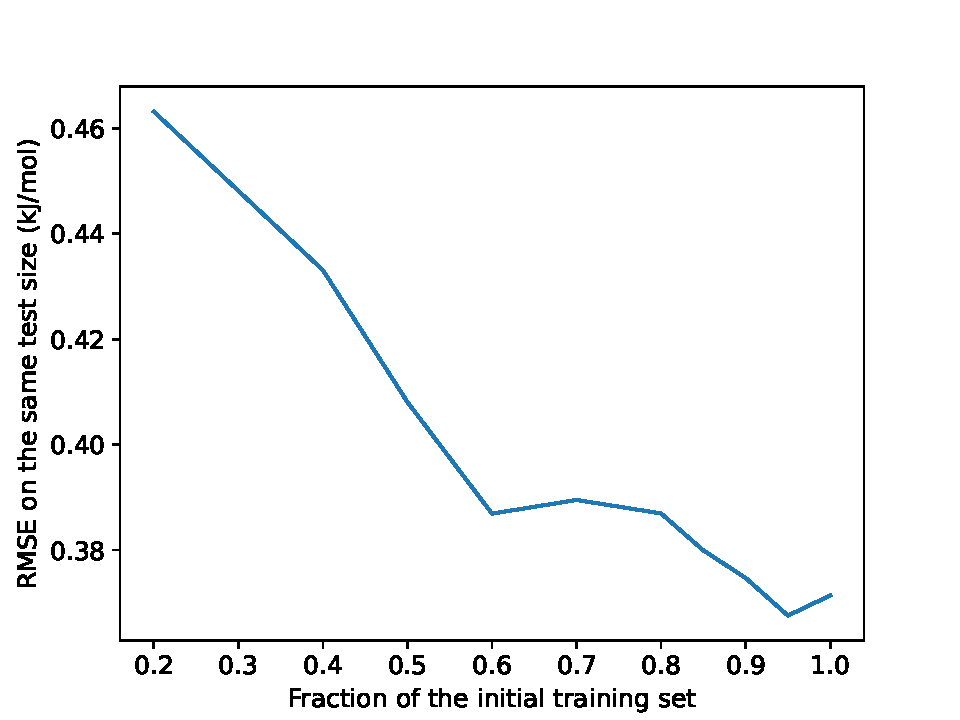
\includegraphics[width=\textwidth]{figures/4-ml/main/training_curve.pdf}
    \caption{Generalization error convergence}\label{fgr:training_curve}
  \end{subfigure}
  \caption{ (a) Scatterplot of the exchange free energy predicted by the model. There is a good agreement between the predicted and true values. On the test set, there is an RMSE of \SI{0.37}{\kilo\joule\per\mole} and an MAE of \SI{0.21}{\kilo\joule\per\mole}. This plot is equivalent to the scatterplot between the logarithm of the ambient-pressure selectivity (Figure~\ref{fgr:S1_prediction}). (b) Root mean squared errors on the same test set (20\% of all data) as a function of the fraction of the training set used to train smaller models. The error decreases as the amount of data increases.}
\end{figure}


To train and fine-tune the parameters of our model, a set of {80\%} randomly chosen structures from the final dataset was defined. A randomized search was conducted over a range of maximum depths, learning rates, sizes of feature samples used by tree and by level, sizes of data samples, and alpha regularization parameters. A set of hyperparameters was selected to minimize the average RMSE computed using a 5-fold cross-validation. The ranges used in the randomized search, as well as the final set of hyperparameters, are provided in section~\ref{sct:hyperparameter}. With this parameterization, our XGBoost model achieved an RMSE of \SI{0.37}{\kilo\joule\per\mole} and an MAE of \SI{0.21}{\kilo\joule\per\mole} on the exchange Gibbs free energies of the test set of 1,616 structures. Converting these results back to selectivity values, the RMSE on the selectivity values would be 2.5, and the logarithm base 10 of the selectivity would have an RMSE of 0.07, indicating a very accurate estimation of the selectivity order of magnitude. To demonstrate that this performance is not coincidental, a 5-fold cross-validation procedure was conducted on the entire dataset, yielding an average RMSE of \SI{0.36}{\kilo\joule\per\mole} with a standard deviation of \SI{0.01}{\kilo\joule\per\mole}, which is consistent with the performance obtained using a standard train/test split.

To assess the possibility of training a better model with an increased amount of training data, models were trained using different fractions of the training set, as depicted in Figure~\ref{fgr:training_curve}. It is observed that the RMSE decreases predictably as the data amount is increased, with stabilization occurring around a fraction of 95\% of the training set. This indicates that the model has sufficient training data to achieve what appears to be the minimum error on this particular test set.

\begin{figure}[ht]
  \centering
    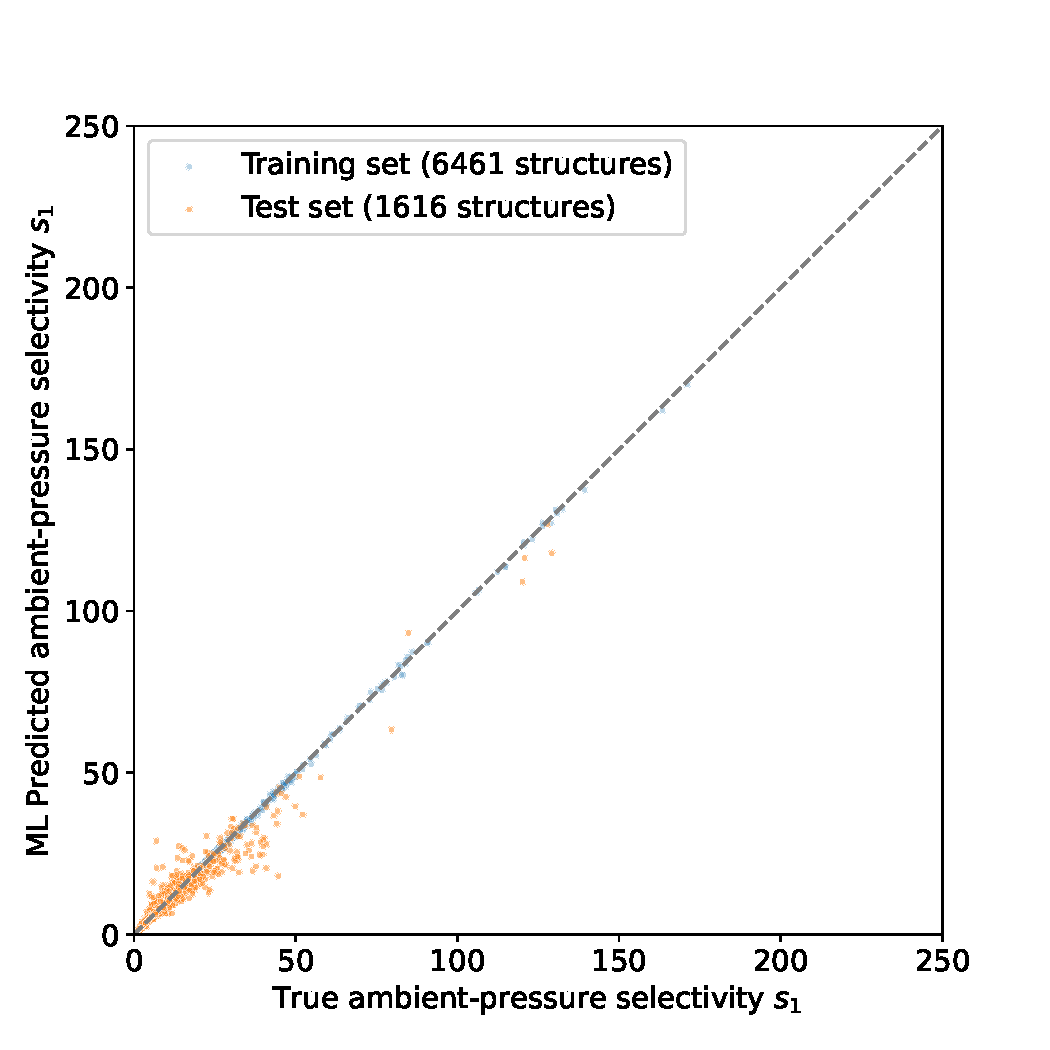
\includegraphics[width=0.48\linewidth]{figures/4-ml/SI_figure/Scatterplot_S1_prediction.pdf}
    \hfill
    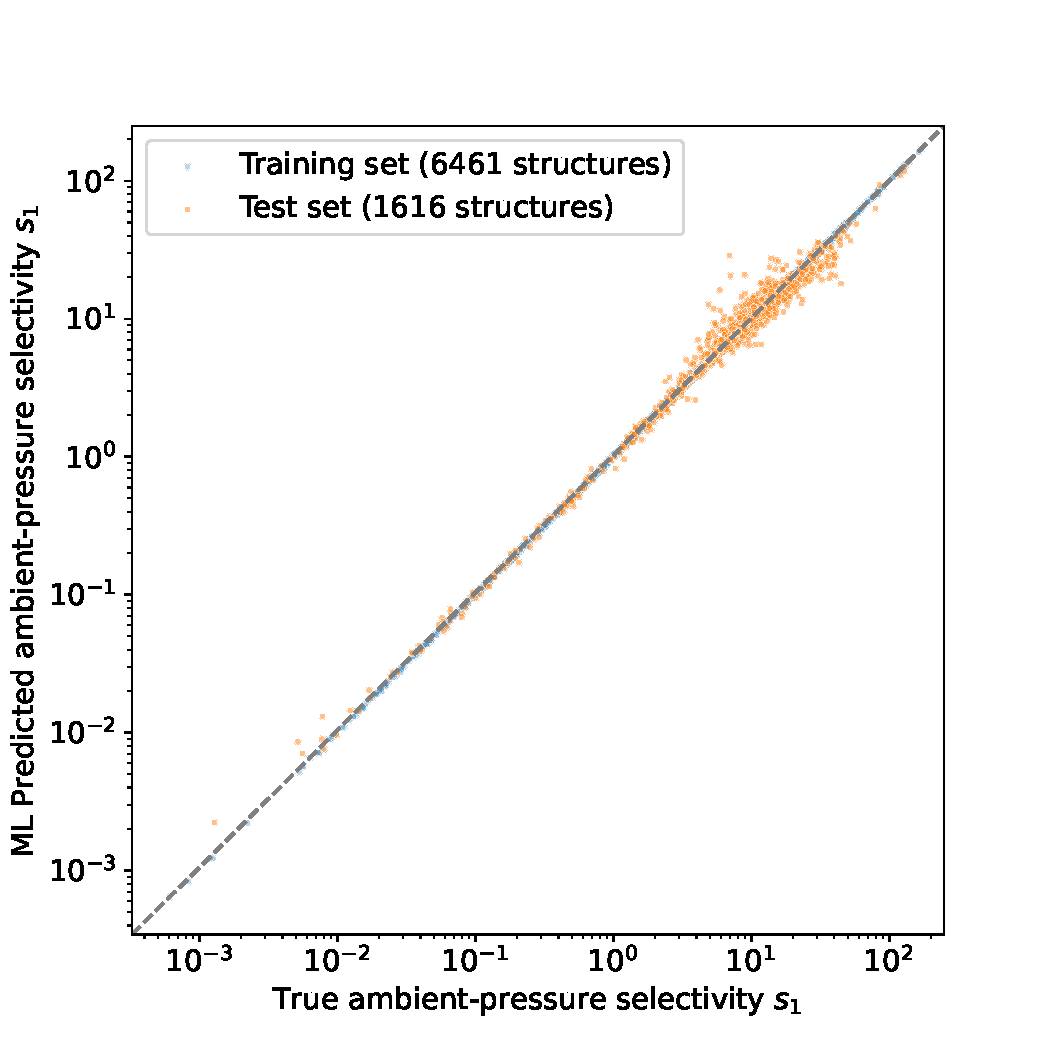
\includegraphics[width=0.48\linewidth]{figures/4-ml/SI_figure/Scatterplot_S1_prediction_logscale.pdf}
    \caption{Scatterplots of the selectivity predicted by the model of ML compared to the selectivity calculated by GCMC in both log and linear scales. The blue points correspond to the training data while the test data is shown in orange. The focus is on the test data since it shows the generalization of the ML model to unseen data. The corresponding errors for the ambient-pressure selectivity are 2.5 and 1.1 for respectively the RMSE and MAE of the selectivity, and 0.065 and 0.038 for the RMSE and MAE of its base-10 logarithm. }\label{fgr:S1_prediction}
  \end{figure}

This method can later be used in a screening procedure that relies on inexpensive descriptors to filter out obviously undesirable structures, retaining only the promising structures for final evaluation by the ML model. To achieve this, as previously explained in the methods section, only 3D MOF structures with an LCD above \SI{4}{\angstrom} are retained, as they possess a positive affinity for xenon, which is a necessary condition for a good Xe/Kr selectivity. Given the excellent predictive performance of the model in this thesis regarding ambient pressure selectivity in structures with good xenon affinity, the proposed screening procedure, illustrated in Figure~\ref{fgr:pipeline}, would include (i) verifying the nature of the structure to ensure it is a 3D MOF structure, (ii) applying a filter based on the LCD value (above \SI{4}{\angstrom}), (iii) performing a pre-evaluation of Xe/Kr selectivity at infinite dilution using the grid-based method, and (iv) conducting the ML evaluation to retain only structures above a certain threshold of ambient-pressure selectivity (\emph{e.g.} 30). Additionally, a more comprehensive assessment of the top structures could be conducted using GCMC simulations, \emph{ab initio} calculations, or adsorption experiments.

\begin{figure}[ht]
\centering
  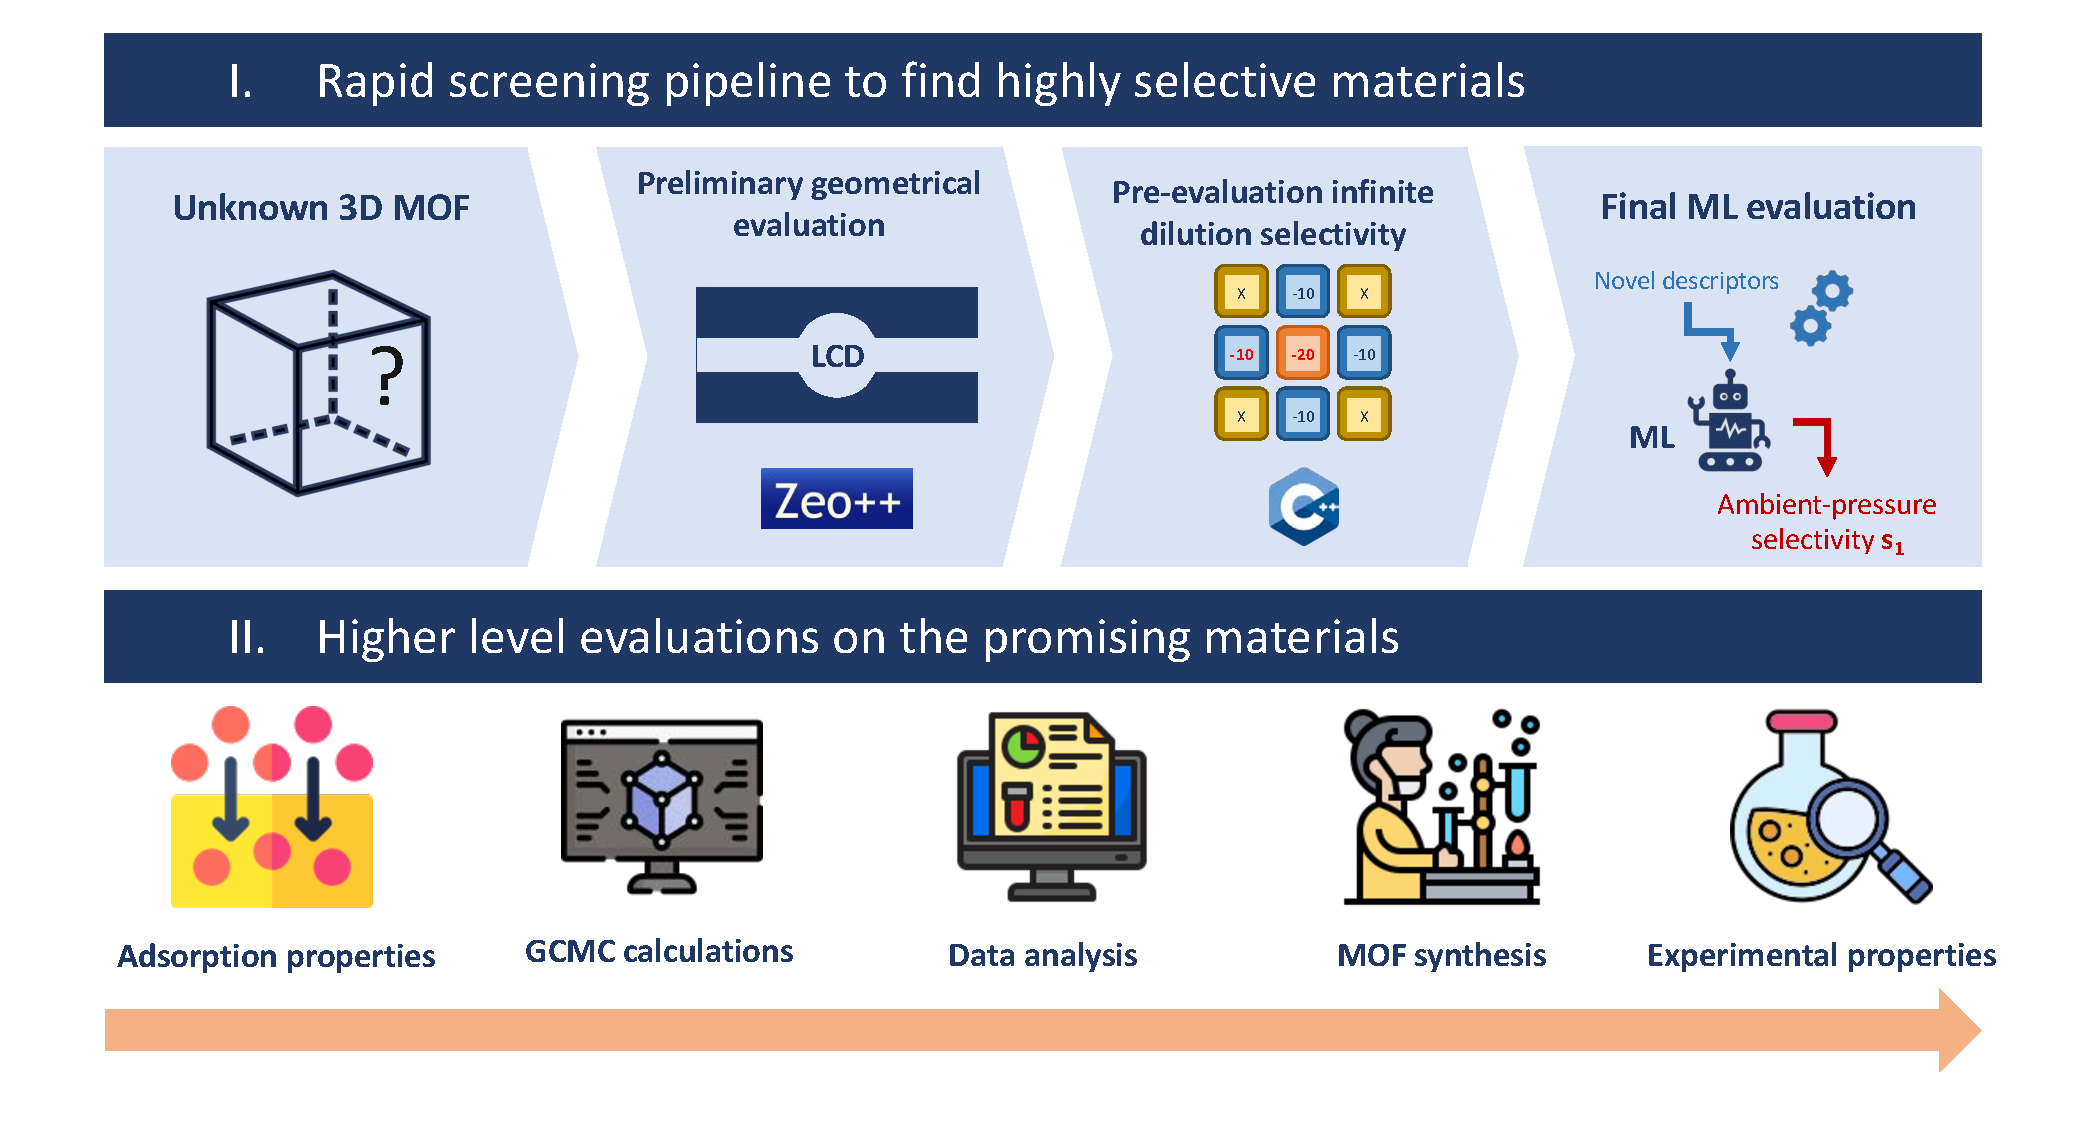
\includegraphics[width=0.99\linewidth]{figures/4-ml/main/pipeline.pdf}
  \caption{An illustration of the screening procedure that could be used to find highly selective materials. The adsorption properties can be rapidly evaluated using structural and energetic conditions on the structure and by confirming it with the ML model. The structures chosen this way can then be tested with higher-level calculations and experiments. }\label{fgr:pipeline}
\end{figure}

\section{Opening the black box}

%% SHAP intro
To gain deeper insights into the reasons behind the selectivity drop, the SHAP library of interpretation models\autocite{SHAP,molnar2020interpretable} are utilized to establish relationships between descriptors and predicted ambient-pressure selectivity. Based on Shapley values\autocite{shapley1953value} which measure the contribution of each descriptor to the prediction, this code facilitates local interpretation of the ML model in this study by disentangling the interdependence between descriptors and extracting individual contributions. To go beyond local interpretation, Shapley values for the entire dataset can be rapidly computed using faster algorithms.\autocite{SHAP} This allows the creation of scatterplots, known as SHAP dependence plots, which depict the contribution as a function of descriptor values and enable a more comprehensive interpretation of our ML model on a global scale. By knowing a descriptor value, it becomes possible to infer, with a certain level of uncertainty, how it influences the final predicted value, thereby shedding light on previously unknown structure--property relationships. Lastly, the mean absolute Shapley values of each feature on the training set were utilized to assess feature importance (Figure~\ref{fgr:featimp_shap}).

\begin{figure}[ht]
  \centering
    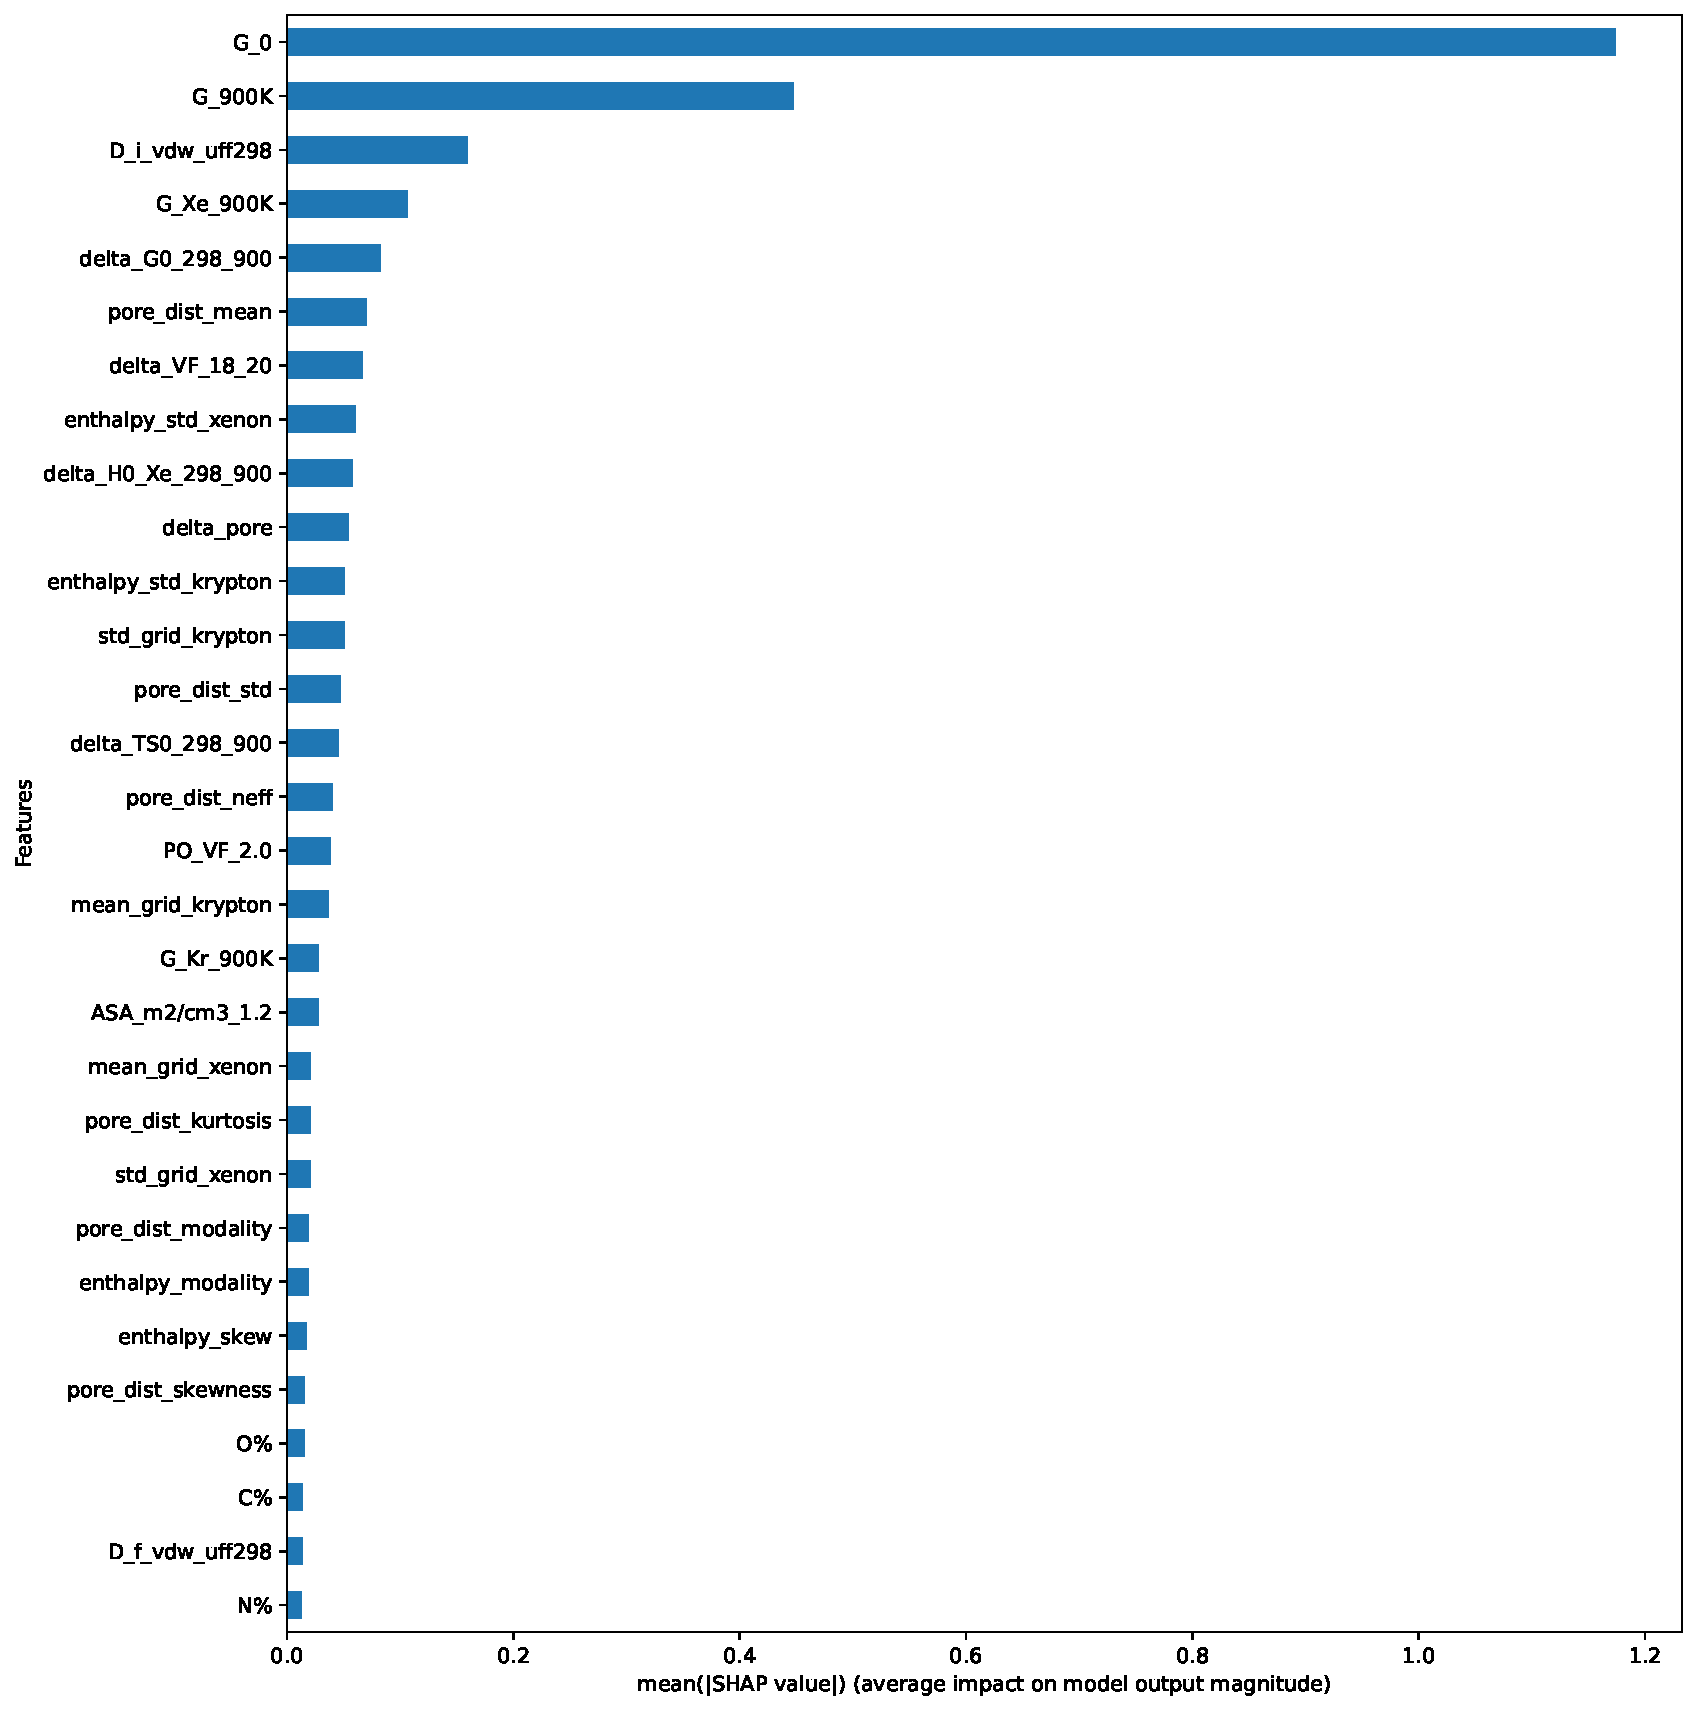
\includegraphics[width=0.70\linewidth]{figures/4-ml/SI_figure/Feature_importance_shapbased.pdf}
    \caption{Barplot of the feature importance for all the descriptors of our final model. The descriptor labels used in this section are explained in more detail in Tables~\ref{tab:geom_descriptors} and~\ref{tab:energy_descriptors}.}\label{fgr:featimp_shap}
  \end{figure}

\subsubsection{Explainable AI}

The final model is trained on the predefined training set using XGBoost with fine-tuned hyperparameters. While evaluating its accuracy on the test set provides valuable insights into the performance of the approach, extracting chemical insights into the hidden relationship between the predicted value and the descriptors also help better understand the thermodynamic origins of the performance. In this work, Shapley values,\autocite{shapley1953value}, a game theory concept developed by Shapley in 1953, is employed to measure the contribution of each descriptor to the predicted value. This tool is used locally to understand how the characteristics of a given structure contribute to the prediction. To establish structure-property relationships, a global interpretation method such as the SHapley Additive exPlanations (SHAP) method, extensively detailed in Christoph Molnar's online book \emph{Interpretable Machine Learning}.\autocite{molnar2020interpretable} The SHAP tool, developed by Lundberg and Lee,~\autocite{SHAP} is based on a faster algorithm adapted to tree-based ML models like gradient boosting, TreeSHAP. It integrates useful global interpretation modules such as SHAP feature importance and dependence plot.

\subsection{Global interpretability}

The descriptors are ranked based on the mean absolute Shapley values of each descriptor to assess their average impact on the model output's magnitude. The importance plot, associated with these values, is presented in Figure~\ref{fgr:featimp_shap}. Although the low-selectivity exchange Gibbs free energy demonstrates significantly higher SHAP importance compared to other descriptors, it serves as a baseline to achieve a correlation similar to that shown in Figure~\ref{fgr:problem}. The other descriptors play a major role in moving the outliers of the figure closer to the diagonal line. Energy descriptors significantly influence the model's predictions, while the geometry-based new descriptors play a secondary yet essential role in assessing the differences between the low-pressure and ambient-pressure cases of interest. To gain a deeper understanding of the mechanisms enabling accurate selectivity prediction by the model --- the RMSE and MAE on the test set's selectivity being respectively $2.5$ and $1.1$. The SHAP dependence plots of each interesting descriptor will be examined, depicting the contribution to the predicted value as a function of the actual descriptor value.

%% Global Interpretability dependence plot
The partial dependence module offered by the SHAP library is applied to provide a comprehensive interpretation of the model. Although other methods, such as partial dependence plots, can be used to compute dependence plots (\emph{e.g.} partial dependence plots),\autocite{molnar2020interpretable}, maintaining a good level of consistency between global and local interpretations by utilizing the same underlying theory is desirable. The SHAP dependence plots for all descriptors in Figures~S9 and S10 exhibit distinct forms, directions, and shapes, which bodes well for the interpretability of the model. Valuable information regarding how the ML model predicts ambient-pressure selectivity was gleaned from the profile of these dependence plots.

%% strong relations
The most important descriptor is the exchange free energy "G\_0" associated with low-pressure selectivity. Its contribution displays a very strong positive linear correlation (Figure~\ref{fgr:pdp_selection}). This descriptor establishes a baseline, on top of which other contributions either decrease the free energy (more selective) or increase it (less selective). The model can be interpreted as a combination of a baseline and smaller adjustments estimating the deviation magnitude from the ideal low dilution case. For instance, the next two descriptors "G\_900K" (\SI{900}{\kelvin} low-pressure exchange free energy) and "G\_Xe\_900K" (\SI{900}{\kelvin} low-pressure xenon adsorption free energy), further contribute to the baseline by providing information on low-pressure selectivity. Moreover, they also offer insights into the deviations necessary to differentiate structures experiencing a drop in selectivity from those maintaining their selectivity. As illustrated in the previous chapter (Figure~\ref{fgr:H_900K} and~\ref{fgr:G_900K}), thermodynamic quantities at high pressure are closer to the \SI{900}{\kelvin} case than to the ambient temperature one. These two descriptors naturally inform the selectivity at higher pressures. In the case of "G\_900K" (Figure~\ref{fgr:pdp_selection}), blue points (corresponding to a "G\_0" of around \SI{-8}{\kilo\joule\per\mole}) can have either negative or negligible contributions, depending on the value. Values below \SI{-4}{\kilo\joule\per\mole} give a negative contribution with a linear relationship, whereas values between $-4$ and \SI{5}{\kilo\joule\per\mole} constantly yield almost zero contributions. This type of domain differentiation illustrates how the model can identify structures with a selectivity drop based on the values of a descriptor. Further examples highlighting the determination of selectivity contributions using the remaining descriptors will be presented.

%% optimal values
The optimal values for the associated descriptors can be highlighted by the U-shape of some SHAP dependence plots. For instance, an optimal value of around $5.1$ is observed for "D\_i\_vdw\_uff298" (Figure~\ref{fgr:pdp_selection}), while the optimal average pore size is approximately $5.6$. These optimal values align with the physical requirement of having  xenon-sized pores to enhance xenon's attraction, as identified in various literature papers. However, it should be noted that these values are slightly higher than those mentioned in the literature due to differences in atom radius definitions.\autocite{Hung_2021} Moreover, values of "delta\_G0\_298\_900" between $4$ and \SI{6}{\kilo\joule\per\mole} (Figure~\ref{fgr:pdp_selection}) have a higher likelihood of contributing negatively, indicating lower ambient-pressure selectivity. These sweet spots provide valuable insights for distinguishing truly selective materials from others. Some SHAP dependence plots have a rather linear domain for the most selective structures (in blue) --- a good linear contribution is observed for the difference of pore volumes between Xe and Kr sized probes "delta\_VF\_18\_20" (Figure~\ref{fgr:pdp_selection}). This implies that a lower void fraction difference corresponds to a more selective structure.  The same trend is observed for the standard deviations of the PSD, denoted as  "pore\_dist\_std", and the Boltzmann weighted krypton interaction energies distribution, referred to as "enthalpy\_std\_krypton". Optimal values for these descriptors tend to be zero. As the value approaches zero, the contribution becomes more negative, indicating a more selective structure at ambient pressure. 

%% optimal domains (weak relations)
In some cases, optimal values are not concentrated around well-identified values but are encompassed within larger domains with threshold values separating them. For instance, the difference between the LCD and the average pore size, denoted as "delta\_pore", has a threshold value around \SI{0.3}{\angstrom}. Below this threshold, the contribution for the most selective structures (blue) is negative (Figure~\ref{fgr:pdp_selection}). Although clear correlations are not evident, a threshold value (of approximately $0.23$) indicates a higher probability of achieving high ambient-pressure selectivity. The same type of domain splits can be observed for the average of the krypton interaction energies distribution "mean\_grid\_krypton" (at around $15$), the Boltzmann weighted xenon interaction energies distribution "enthalpy\_std\_xenon" (at around $2.5$), the difference of exchange entropic term between ambient temperature "delta\_TS0\_298\_900" (at around $3$) and high temperature, and the effective number associated with the PSD "pore\_dist\_neff" (at around $2.3$). These domains serve to distinguish structures with a selectivity drop at ambient pressure from those without, particularly important for identifying selective structures at low pressure.

\begin{figure}[ht]
\centering
  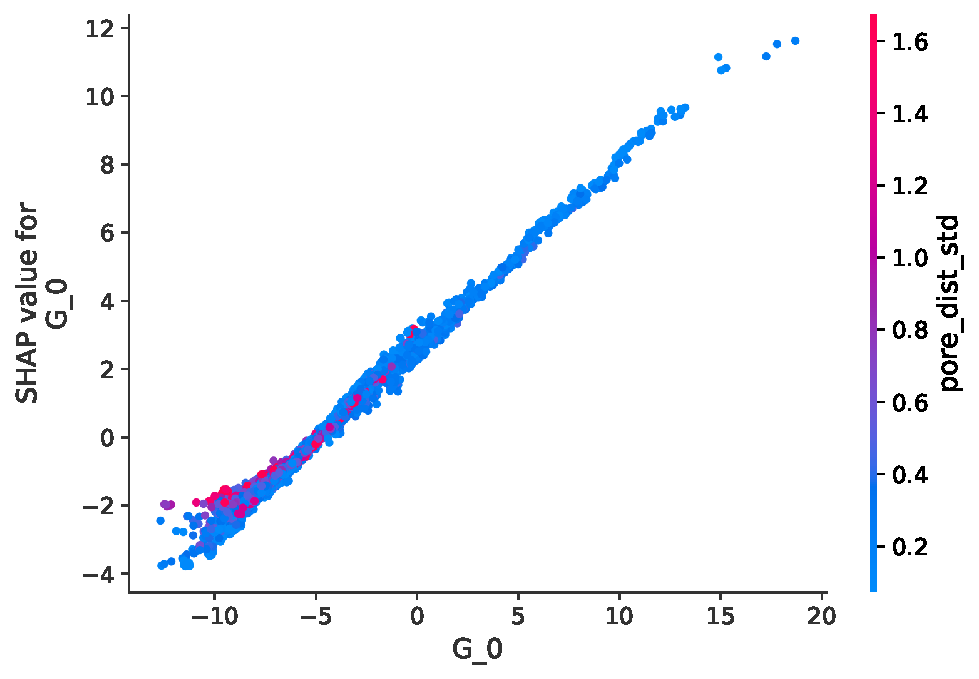
\includegraphics[width=0.32\linewidth]{figures/4-ml/SDP/G_0.pdf}
  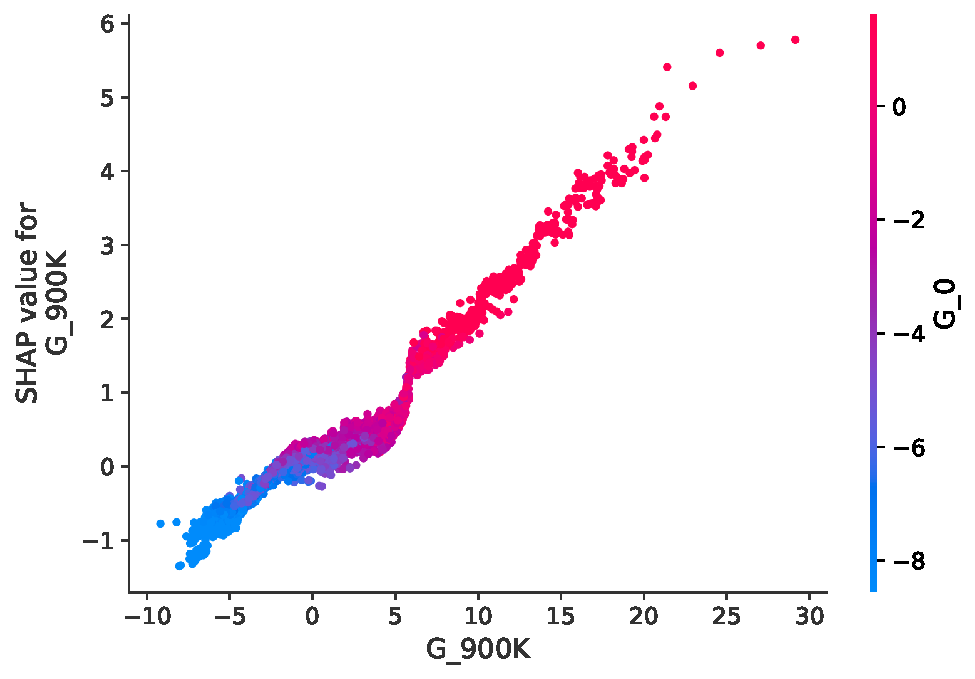
\includegraphics[width=0.32\linewidth]{figures/4-ml/SDP/G_900K.pdf}
  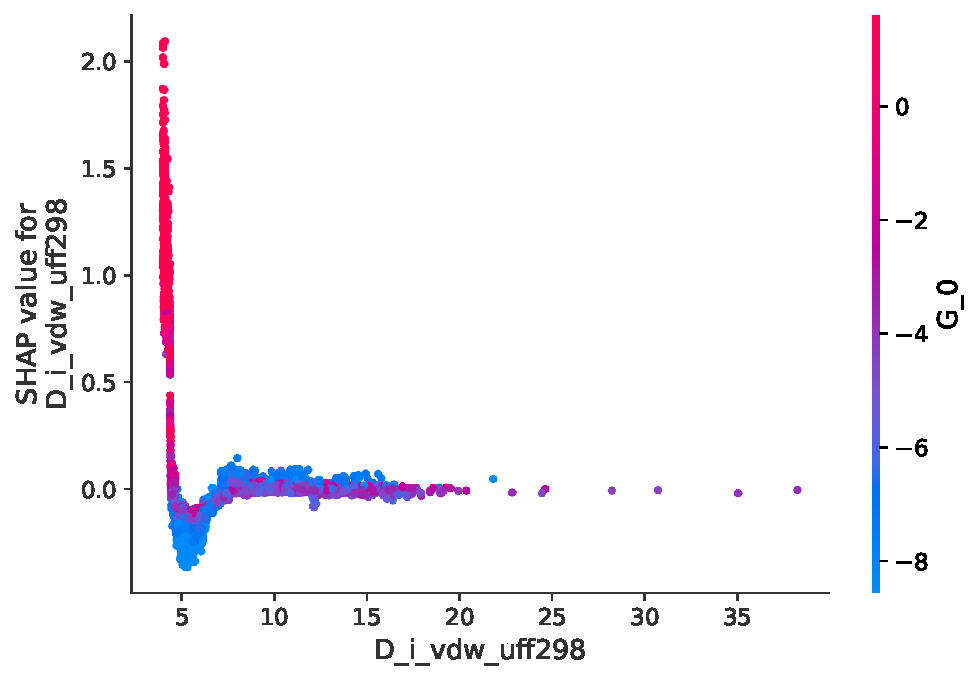
\includegraphics[width=0.32\linewidth]{figures/4-ml/SDP/D_i_vdw_uff298.pdf}
  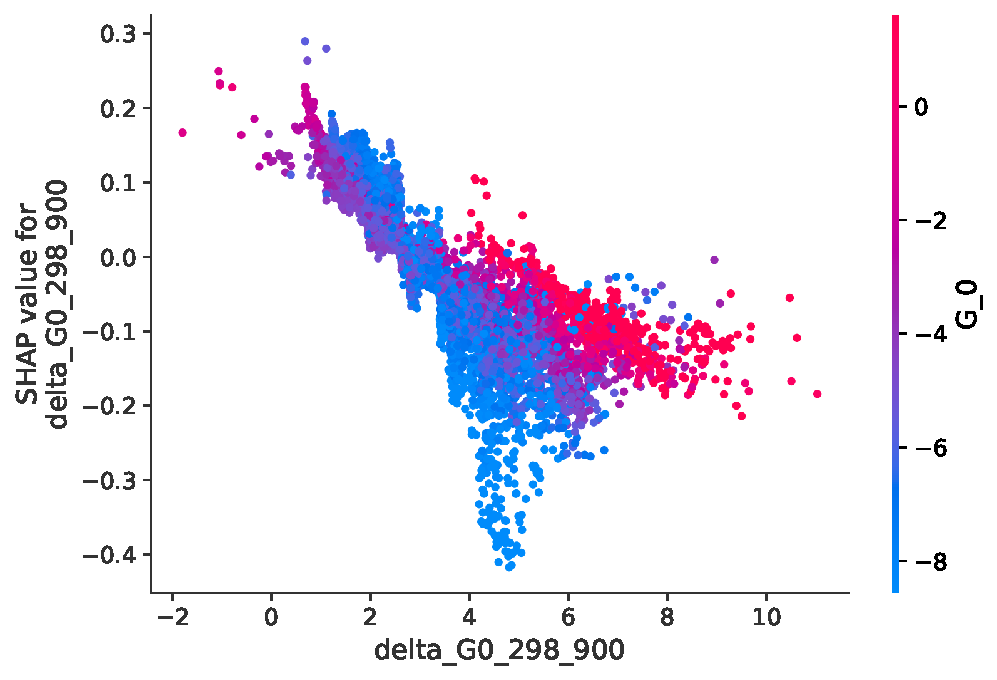
\includegraphics[width=0.32\linewidth]{figures/4-ml/SDP/delta_G0_298_900.pdf}
  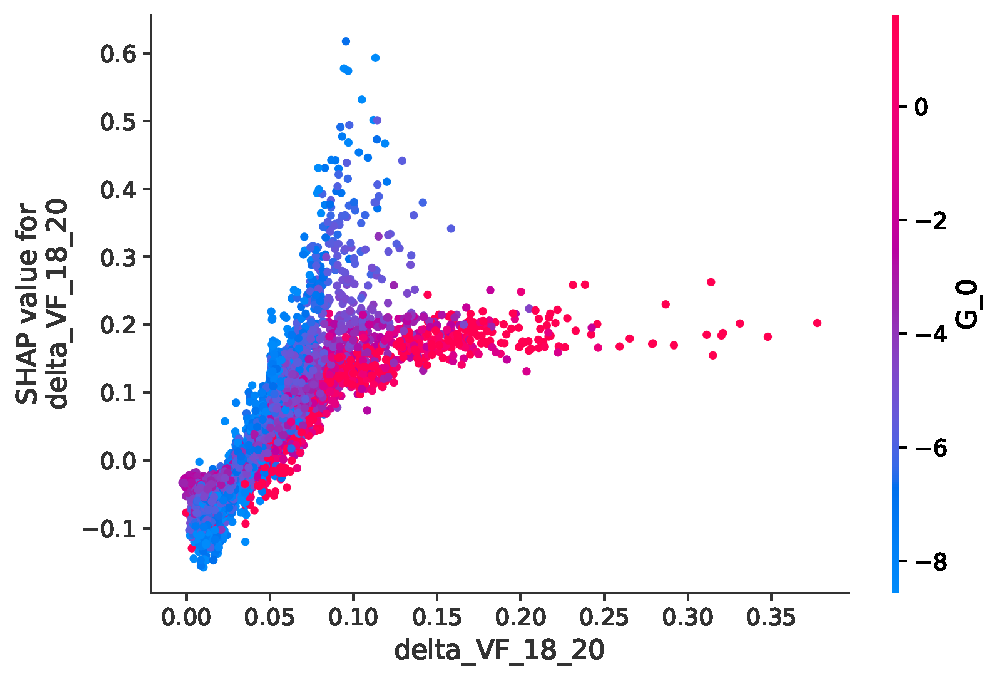
\includegraphics[width=0.32\linewidth]{figures/4-ml/SDP/delta_VF_18_20.pdf}
  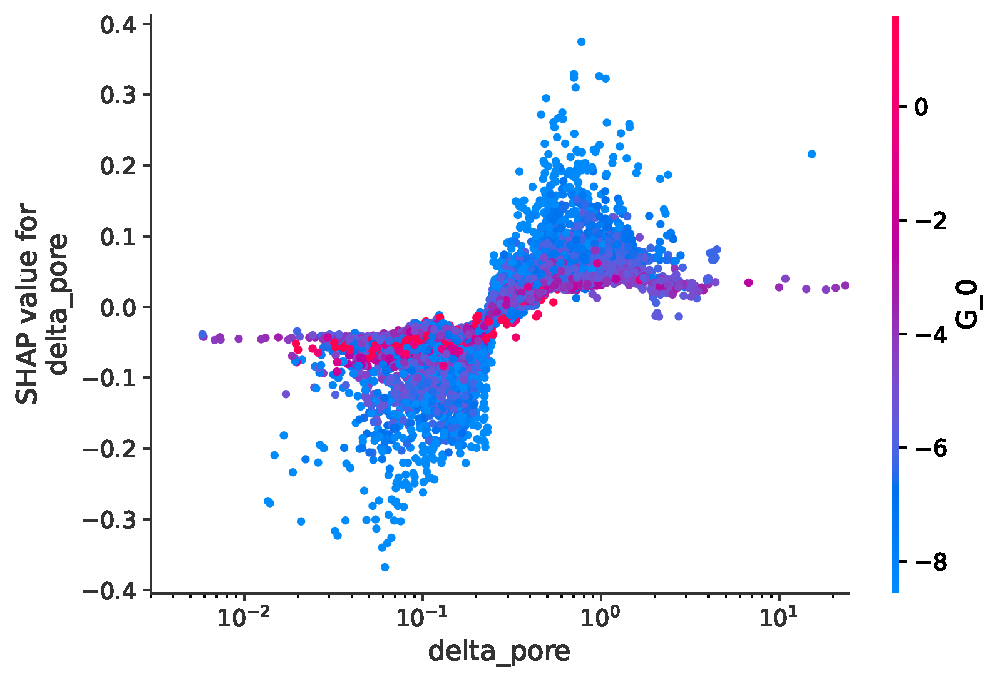
\includegraphics[width=0.32\linewidth]{figures/4-ml/SDP/delta_pore.pdf}
\caption{ Some relevant SHAP dependence plots that are provided here. A SHAP dependence plot corresponds to the Shapley values as a function of the feature values for all structures of the dataset. These SHAP plots show the contribution of the features to the prediction given by the ML model. Each Shapley value depends not only on the value of the feature itself but also on the values of other features. For this reason, the plots are labeled by a relevant second feature. }\label{fgr:pdp_selection}
\end{figure}

\subsection{Local interpretability}

%% local interpretation
To apply the previous analysis in practice, archetypal structures and their selectivity predictions based on descriptor values will be examined. Two MOF structures from the test set, with CSD codes \texttt{VIWMIZ} and \texttt{BIMDIL}, are chosen. Both structures are selective at low pressure, but the first one decreases in selectivity while the second one maintains it at ambient pressure. The focus will be on understanding how the model distinguishes between these two completely distinct behaviors.

\texttt{VIWMIZ} belongs to the category of highly selective structures that undergo a selectivity drop at ambient pressure. When converting the free energy values to selectivity values, \texttt{VIWMIZ} has a selectivity of $62.8$ at infinite dilution and $14.5$ at ambient pressure. The ML model successfully predicts a close value of $12.0$ for the ambient-pressure selectivity based on the given descriptor values. Specifically, the descriptor "G\_0" has a highly negative value, which explains its relatively high negative contribution of $-1.81$. However, the contribution of "G\_900K" is relatively low at $-0.57$ compared to other materials (Figure~\ref{fgr:pdp_selection}), as a value of $-4.05$ is not the most negative among all structures. Conversely, the remaining descriptors have positive contributions, which lead to the selectivity drop. For instance, the difference in pore sizes, "delta\_pore", has a value of \SI{1.38}{\angstrom} (above the threshold of \SI{0.23}{\angstrom}), which contributes $+0.25$ to the predicted selectivity. This value aligns with the value ranges observed in the associated dependence plot. Similar analyses can be performed on the positive contributions of other descriptors shown in Figure~\ref{fgr:contribution} by referring to the dependence plots: "pore\_dist\_std" is above the threshold of $0.4$, "enthalpy\_std\_krypton" is above \SI{2.5}{\kilo\joule\per\mole}, "pore\_dist\_neff" is above $2.3$, "delta\_TS0\_298\_900" falls below \SI{3}{\kilo\joule\per\mole} and "enthalpy\_modality" is around $0.75$ where positive contributions are more commonly observed. However, the "delta\_G0\_298\_900" value is somewhat close to its optimal value, resulting in a negative contribution in this specific prediction. The remaining features have negligible contributions. Analyzing the contributions of each descriptor to the prediction given by the model of this work helps understanding the underlying features of the \texttt{VIWMIZ} structure that explain the selectivity drop at higher pressure. Descriptors such as the shape of the xenon and krypton energy distributions ("enthalpy\_std\_krypton" and "enthalpy\_modality") and the PSD ("pore\_dist\_std" and "pore\_dist\_neff" ) as well as the void fraction difference "delta\_pore" play key roles in the lower selectivity at ambient pressure compared to the ideal infinite dilution case. Intuitively, an effective number of pores exceeding 2 suggests the presence of different pore sizes, which aligns with the presence of less attractive pores for xenon, ultimately leading to decreased selectivity. This observation is consistent with a high standard deviation of the PSD or the Boltzmann-weighted krypton interaction energy distribution. Furthermore, a significant difference between the average pore size and the LCD indicates a disparity in pore sizes, resulting in larger pores that become increasingly loaded as pressure rises. However, interpreting the entropic term is more complex and presents unexplored ways of addressing the selectivity drop at higher pressure, as revealed in the previous study (chapter 2).

\begin{figure}[ht]
    \centering
    \begin{subfigure}[b]{0.47\textwidth}
      \centering
      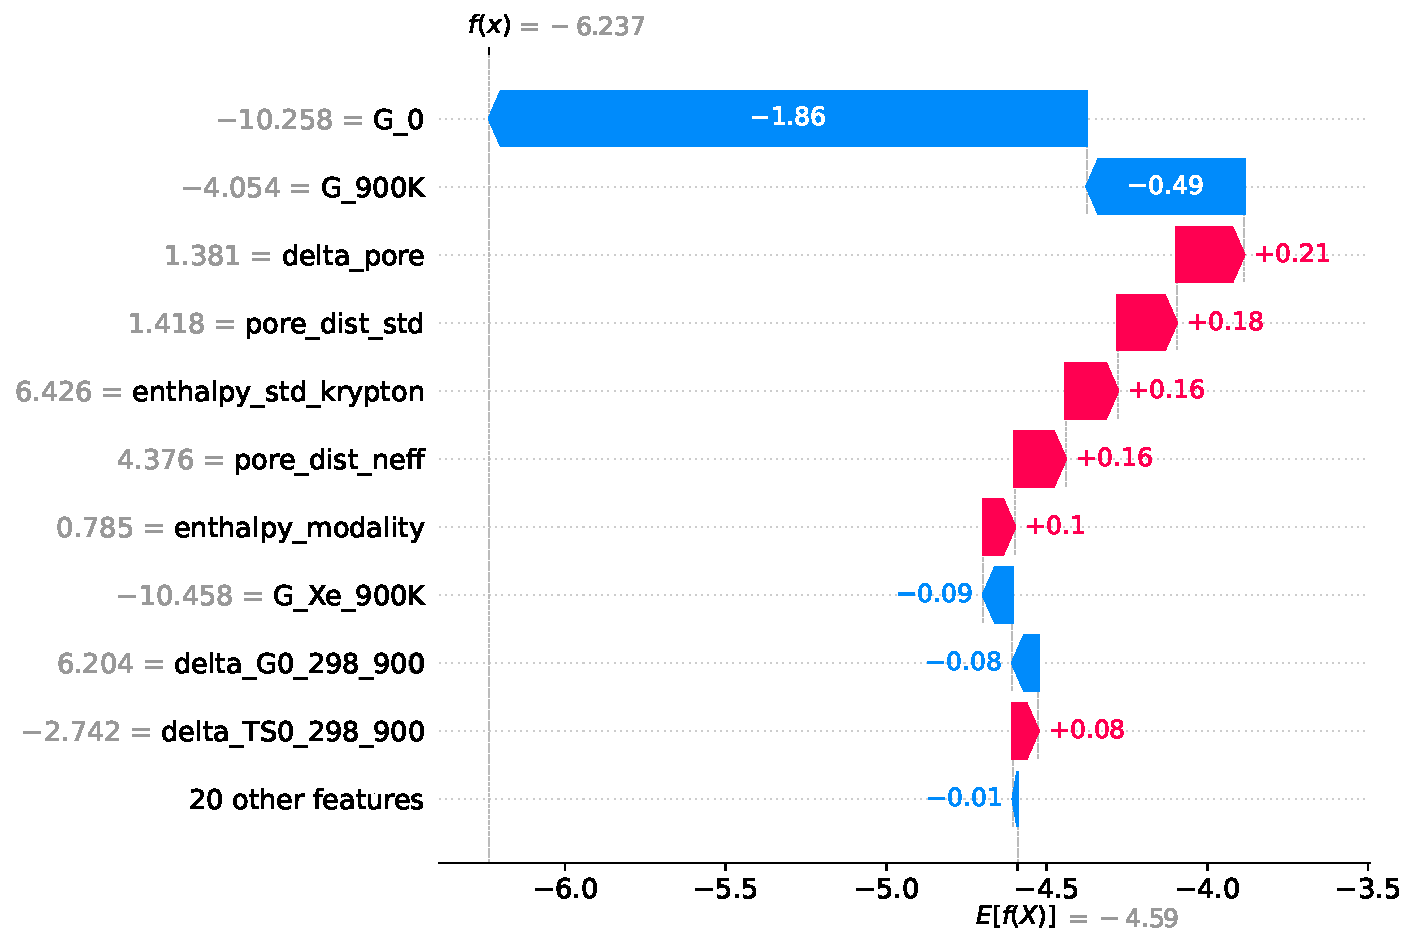
\includegraphics[width=\textwidth]{figures/4-ml/main/VIWMIZ_clean.pdf}
      \caption{\texttt{VIWMIZ}: true $\Delta\e{exc} G_1=-6.63$}
    \end{subfigure}
         \hfill
    \begin{subfigure}[b]{0.47\textwidth}
      \centering
      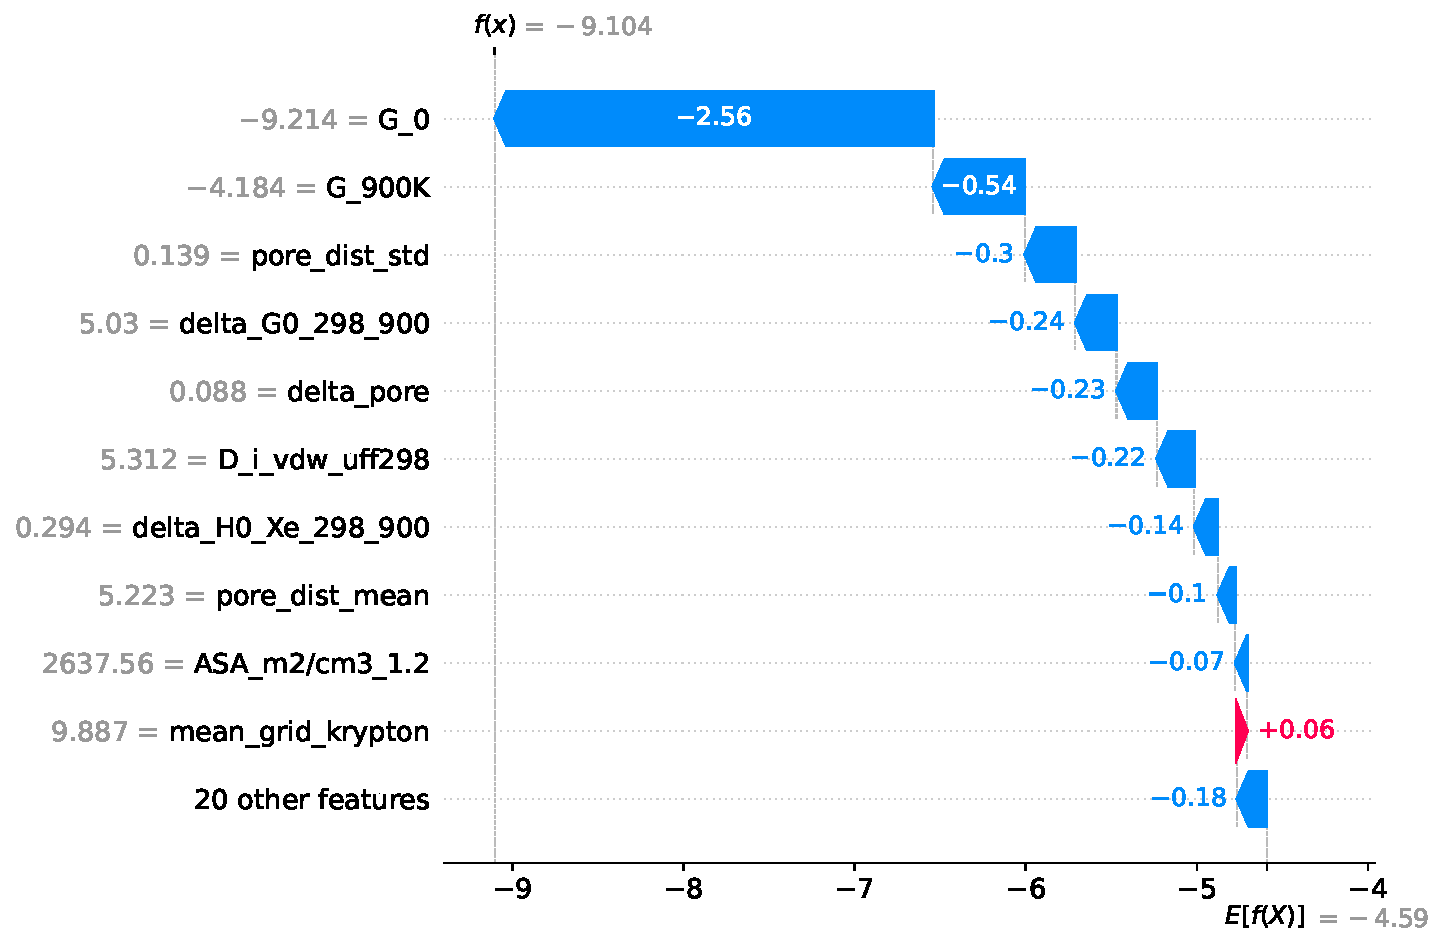
\includegraphics[width=\textwidth]{figures/4-ml/main/BIMDIL_clean.pdf}
      \caption{\texttt{BIMDIL}: true $\Delta\e{exc} G_1=-9.20$}
    \end{subfigure}
  \caption{Main contributions of the descriptors on the selectivity prediction of two archetypal examples. The descriptor labels used are detailed in Table~\ref{tab:geom_descriptors} and~\ref{tab:energy_descriptors}.}\label{fgr:contribution}
\end{figure}

The second structure \texttt{BIMDIL} is also among the most selective with a selectivity at low pressure of $41.0$, while maintaining it to $41.2$ at ambient pressure. The stability of the selectivity is accurately predicted by assigning a value of $40.0$. Consequently, the first contribution of "G\_0" is one of the most negative contributions, establishing a baseline of $-2.4$ for subsequent contributions. Although the contributions of "G\_900K" and "G\_900K", they continue to decrease the predicted selectivity value. The joint contributions of other descriptors will discriminate between the two structures and determine why this particular structure will maintain its selectivity. In contrast to the previously analyzed structure, this structure has a "delta\_pore" value below \SI{0.3}{\angstrom}, explaining its negative Shapley value in the prediction of this study. The contribution of "delta\_G0\_298\_900", which had only a slightly negative impact on the other structure, now plays a significant role as it falls within the range of $4$ to \SI{6}{\kilo\joule\per\mole} (Figure~\ref{fgr:contribution}). Additionally, it is observed that "pore\_dist\_std" is below the threshold, in contrast to the previous structure where it was above the threshold. Furthermore, the other contributions align with the rules suggested by the SHAP dependence plots, and no apparent anomalies are detected. The combined effects of all the descriptors result in a lower free energy value, leading to the conservation of selectivity at higher pressure. The set of descriptor values for this structure significantly differs from the previous one, with many values contributing to opposite domains. This disparity allows the model to differentiate between highly selective structures and identify those that will maintain their selectivity at higher pressure.

%% conclusions + sum-up of some qualitative rules
These two examples provide a deeper understanding of how the model distinguishes structures that lose selectivity at higher pressure from those that do not. Most dependence plots exhibit a strong association between descriptors and their effects, with outliers being rare enough to comprehend the internal logic of the model. As previously discussed, the first three descriptors establish a baseline for the observed selectivity drop with limited information. Subsequently, the contributions of other descriptors can be positive, negligible, or negative depending on the domain where the values of the descriptor lie. For instance, the average pore size and largest cavity diameter need to be within specific ranges to maximize the likelihood of maintaining selectivity at higher pressure, aligning with previous studies emphasizing the importance of pore sizes similar to xenon for Xe/Kr separation. The difference in entropy between ambient temperature and \SI{900}{\kelvin} is a surprising descriptor that separates selective structures based on whether its value falls within a specified range. Similarly, the difference in void fraction occupied by xenon and krypton is intriguing as it impacts selectivity differently depending on whether the structure is highly selective or not, with the contribution being more or less proportional to its value. Various methods of measuring the disparity of the PSD and interaction energy distribution play a key role in identifying highly selective structures (indicated in blue on the dependence plot in Figure~\ref{fgr:pdp_selection}) that either maintain or decrease in selectivity. These methods include calculating the difference between the average pore size and the LCD, as well as the standard deviation of the PSD or Boltzmann-weighted energy distribution, which exhibit distinct behaviors based on the domain in which the value lies. The SHAP dependence plots provide valuable insights into the mechanisms underlying the ML model presented in this thesis and, more broadly, shed light on the understanding of Xe/Kr separation origins.

\section{Beyond thermodynamic considerations}

To gain a deeper understanding of separation processes within nanoporous materials, a machine learning prediction of Xe/Kr ambient-pressure selectivity was performed, aiming for faster results compared to standard GCMC calculations. The CoRE MOF 2019 database was utilized for MOF structures, enabling the evaluation of xenon/krypton selectivity in less than a minute, whereas an equivalent GCMC calculation typically requires approximately \SI{40}{\minute}. 
Unlike the majority of selectivity predictions in the literature, the decision was made to predict selectivity on a logarithmic scale that focuses on the order of magnitude rather than the exact value of selectivity for highly selective materials. Moreover, converting to an exchange Gibbs free energy allowed for a more thermodynamic approach based on enthalpy, entropy, and free energy values. The challenge consisted of predicting the free energy equivalent of ambient-pressure selectivity using low-pressure selectivity alongside key energy, geometrical and chemical descriptors. The resulting fully optimized ML model exhibited high performance, yielding an RMSE of \SI{0.36}{\kilo\joule\per\mole}, which corresponds to an RMSE of $0.06$ on the base-10 log of selectivity.

One specific objective was to uncover the underlying reasons for the observed selectivity drop at high pressure in certain highly selective materials at low pressure. initially studied in chapter 2. Previous studies (chapter 2) found that high diversity of pore sizes and channel sizes that favor adsorbate reorganizations could be at the origin of this phenomenon. Through the application of interpretability tools, quantitative factors explaining the conservation or decrease in selectivity for highly selective materials were identified. Depending on energy averaging at \SI{900}{\kelvin}, statistical characterizations of energy or pore size distributions, and differences in occupiable volumes, a structure could exhibit either a selectivity similar to the infinite dilution case or a substantially lower selectivity at higher pressure. The XGBoost model employed in this study utilizes a complex ensemble of decision trees to capture the quantitative rules that can be extracted from the model and used to establish heuristics supporting the intuition about Xe/Kr selectivity in MOF structures.

%% Framework could be reproduced for other type of applications
The final ML model could be used in a well-designed workflow to find the best performing materials. For instance, structures with pores that are unable to accommodate xenon could be filtered out, followed by the application of a low-pressure selectivity calculation to eliminate selectivity values below a specified threshold. Finally, the structures that would encounter a drop in selectivity could be removed using the model. As a proof of concept, the methodology was tested on Xe/Kr separation, which represents one of the simplest adsorption systems (monoatomic species and the absence of electrostatic interactions). A similar approach could be generalized to other separation applications by calculating the infinite dilution energies with a more conventional method (\emph{e.g.} Widom's insertion), while adjusting the definitions of descriptors to suit the adsorbates of interest.

%% Drawbacks + perspectives
The ambition of this study was to introduce new descriptor ideas that contribute to the development of increasingly efficient screening methodologies for identifying optimal materials for specific applications. However, similar to other studies in this field, the simulations in this study relied on a set of strong assumptions, wherein rigid frameworks and non-polarized classical forcefields were employed. Previous literature suggested that the design of the most selective materials for Xe/Kr separation were synthesized based on the effect of open-metal sites, leveraging the difference in polarizability between the two molecules to achieve efficient separation.\autocite{Li_2019, Pei_2022} Moreover, the flexibility of structures could be achieved by employing flexible forcefields with appropriate simulation methodologies\autocite{Bousquet2012} or by conducting multiple rigid simulations using snapshots from NPT simulations\autocite{Witman_2017}. The simulations could be enhanced at the cost of CPU time by coupling them with a reduction in simulation time, such as the one presented in this chapter. The pursuit of ever-faster evaluation tools enabled the exploration of more complex properties and the discovery of structures with increasingly relevant characteristics. Further discussion on these potential improvements will be presented in greater detail in Chapter 6.

\vspace{1cm}

The next chapter will focus on another shortcoming of the simple thermodynamic approach, namely the consideration of kinetic limitations in the screening process. In the problem of adsorbent-material separation, the transport effect does not play a key role in evaluating the separation performance of the material. Instead, it serves as a constraint that could potentially affect the performance of some seemingly top materials. Various methodologies will be examined to incorporate these transport properties, which are computationally demanding and challenging to obtain experimentally.

\OnlyInSubfile{\printglobalbibliography}

\end{document}
